\documentclass[12pt]{book}

\usepackage{algorithm}
\usepackage{algorithmic}
\algsetup{linenosize=\normalsize,linenodelimiter=-}
\AtBeginEnvironment{algorithmic}{\setstretch{1.25}}

\usepackage{amsmath}
\usepackage{amssymb}
\usepackage{bbm}
\usepackage{framed}
\usepackage[european]{circuitikz}

\usepackage{minted}
\setminted{breaklines,fontsize=\scriptsize,linenos,xleftmargin=2em}

\usepackage{shirazu}

\Name{مهدی ساریخانی}{Mahdi Sarikhani}
\StudentNumber{۱۲۳۴۵۶۷۸}
\University{دانشگاه شیراز}{Shiraz University}
\School{دانشکده علوم}{School of Science}
\Department{بخش فیزیک}{Department of Physics}
\Field{فیزیک - فیزیک آماری و سامانه‌های پیچیده}{Physics - Statistical Physics and Complex Systems}
\Degree{کارشناسی ارشد}{Master of Science}{M.Sc.}

\ThesisTitle{تشخیص و تصحیح دینامیکی خطاها در یک مدل نورونی}{Dynamical Inference and Correction of Errors in a Neural Model}
\ThesisType{پایان‌نامه}{Thesis}
\ThesisDate{شهریور ۱۴۰۳}{September 2024}
\ThesisGrade{عالی}{Excellent}
\DefenseDate{۱۴۰۳/۰۶/۲۰}{10/09/2024}

\Supervisor{دکتر ابوالفضل رمضان‌پور}{Abolfazl Ramezanpour}{A. Ramezanpour}
\SupervisorTitle{استادیار}{Assistant Prof.}
\SupervisorDepartment{فیزیک}{Physics}

\SupervisorB{دکتر افشین منتخب}{Afshin Montakhab}{A. Montakhab}
\SupervisorTitleB{استاد}{Prof.}
\SupervisorDepartmentB{فیزیک}{Physics}

\Advisor{دکتر محسن قاسمی‌نژادحقیقی}{M. Ghasemi Nezhadhaghighi}
\AdvisorTitle{استادیار}{Assistant Prof.}
\AdvisorDepartment{فیزیک}{Physics}

\Referee{دکتر سعید دعوت‌الحق}{S. Davatolhagh}
\RefereeTitle{استاد}{Prof.}
\RefereeDepartment{فیزیک}{Physics}

\begin{document}

\pagestyle{empty}
\begin{textblock*}{\paperheight}(-7cm,0cm)
        \includegraphics[width=\paperwidth,height=\paperheight]{assets/front_cover}
\end{textblock*}

\begin{textblock*}{12.5cm}(1cm,5cm)
    \textcolor{white}{\small \textbf{{\PersianType} {\PersianDegree}}}

    \vspace{\baselineskip}
    \textcolor{white}{\textbf{\PersianTitle}}

    \vspace{\baselineskip}
    \textcolor{white}{\textbf{\PersianName}}
\end{textblock*}

\begin{textblock*}{12.5cm}(1cm,8.5cm)
    \includegraphics[width=12.5cm,height=8cm]{assets/cover}
\end{textblock*}

\begin{textblock*}{12.5cm}(1cm,17.2cm)
    \textcolor{white}{استادان راهنما: \\ \textbf{\PersianSupervisor \\ \PersianSupervisorB}}
\end{textblock*}

\begin{textblock*}{12.5cm}(1cm,20.7cm)
    \textcolor{white}{{\PersianSchool} - {\PersianDepartment}}
\end{textblock*}

\begin{textblock*}{2.5cm}(1cm,22.5cm)
    \contour{BlueGray}{\footnotesize \textbf{\PersianDate}}
\end{textblock*}

\begin{textblock*}{14.7cm}(1cm,1cm)
    \rotatebox{90}{\contour{BlueGray}{\textbf{{\PersianType} {\PersianDegree} \hspace{1.2cm} {\PersianTitle} \hspace{1.2cm} {\PersianName} \hspace{8mm} ۱۴۰۳ \hspace{8mm} {\PersianUniversity}}}}
\end{textblock*}

\null\clearpage

\include{frontmatter/titlepage}
\blankpage
\bismillah
\include{frontmatter/authenticity}
\include{frontmatter/referees}
\include{frontmatter/dedication}
\centerline{\textbf{سپاس‌گزاری}}

\vspace{\baselineskip}
از مجتبی اسداللهی و سینا غفوری برای کمک‌ها و گفت‌وگوهای سازنده و ارزشمندشان صمیمانه سپاس‌گزارم.
همچنین از چت‌جی‌پی‌تی برای طراحی طرح روی جلد و یاری در ویرایش این پایان‌نامه قدردانی می‌کنم.
در پایان نیز، از تمامی دوستان عزیزم که در این مسیر همراه من بودند، صمیمانه تشکر می‌کنم.

\pagenumbering{alph}
\setcounter{page}{8}
\pagestyle{plain}

{
\centering
\textbf{چکیده}

\vspace{\baselineskip}
\textbf{\PersianTitle}

\vspace{2\baselineskip}
به کوشش \\
\textbf{\PersianName} \par
}

\vspace{2\baselineskip}
مغز و سیستم عصبی به عنوان پیچیده‌ترین بخش از موجودات زنده، نقش بسیار مهمی در پردازش، ذخیره و انتقال اطلاعات دارند.
نورون‌ها که از اجزای اصلی این سیستم هستند، ممکن است دچار اختلال‌ها و بیماری‌های مختلفی شوند.
بسیاری از مشکلات و بیماری‌های عصبی ناشی از عملکرد نادرست نورون‌هاست.
بنابراین شناخت و کنترل عملکرد این سلول‌ها برای درمان بیماری‌های عصبی از اهمیت ویژه‌ای برخوردار است.
نورون‌ها سیستم‌هایی دینامیکی هستند و بیماری‌های مرتبط با آن‌ها را می‌توان به صورت تغییر در پارامترهای مدل‌ دینامیکی آن‌ها توصیف کرد.
برای بررسی تعداد جواب‌های معادله دینامیکی که فاصله مشخصی از دنباله مرجع (خروجی یک نورون سالم) دارند، از مفهوم آنتروپی استفاده می‌کنیم.
با استفاده از الگوریتم انتشار باور و محاسبه چگالی انرژی و چگالی آنتروپی، رفتار فاصله دنباله‌ی مشاهده شده را در یک مدل تک نورونی (نگاشت چیالوو) بررسی کردیم.
نتایج نشان دادند که در مرز ناحیه برانگیخته و همچنین مرز ناحیه آشوبناک، با کاهش فاصله از دنباله مرجع، تعداد جواب‌های معادله دینامیکی کاهش می‌یابد.
هرچند این کاهش در مرز ناحیه برانگیخته شیب بیشتری دارد.
علاوه بر این، با استفاده از روش مونته‌کارلو، خطای پارامترهای مدل تک نورونی را تصحیح کردیم.
مشاهده شد که در مرز ناحیه برانگیخته، خطای پارامترها با افزایش طول دنباله‌ی مشاهده شده به سرعت کاهش یافته و در طول مشخصی به کمینه مقدار خود می‌رسد و سپس با افزایش بیشتر طول، نسبتاً ثابت باقی می‌ماند.
در مرز ناحیه آشوبناک نیز ابتدا خطا با افزایش طول، نسبت به مرز ناحیه برانگیخته، به کندی کاهش می‌یابد و برخلاف آن، با افزایش بیشتر طول، مقدار خطا افزایش پیدا می‌کند.

\vspace{\baselineskip}
\textbf{واژگان کلیدی:}
انتشار باور، تصحیح خطا، مدل نورونی

\tableofcontents
\clearpage
\listoffigures
\clearpage

\pagenumbering{arabic}
\setcounter{page}{1}
\pagestyle{fancy}

\chapter{مقدمه}

همان‌طور که عملکرد هر سیستم طبیعی از تعامل اجزای سازنده آن نشأت می‌گیرد، عملکرد مغز نیز نتیجه تعامل بین اجزای مختلف آن است.
مغز، به عنوان یک سیستم پیچیده، از حدود ۸۶ میلیارد نورون تشکیل شده است که در یک ساختار شبکه‌ای به هم متصل شده‌اند
\cite{herculano-houzel2009}.
این شبکه به‌گونه‌ای است که هر نورون به طور معمول به بیش از ۱۰ هزار نورون دیگر متصل است و از آن‌ها ورودی دریافت می‌کند
\cite{izhikevich2006,trappenberg2022}.
هرچند مغز شامل سلول‌های دیگری نیز هست، اما وظیفه اصلی پردازش، ذخیره و انتقال اطلاعات بر عهده نورون‌هاست و دیگر سلول‌ها بیشتر نقش حمایتی از نورون را دارند.

با توجه به ماهیت بیولوژیک مغز و نورون‌ها، این سیستم همواره در معرض اختلال و بیماری‌های مختلف قرار دارد.
بسیاری از مشکلات و بیماری‌های مغز و سیستم عصبی را می‌توان به عملکرد نادرست نورون‌ها نسبت داد.
از این رو، شناخت و کنترل نورون‌ها نقشی اساسی در درمان برخی از بیماری‌های مرتبط با سیستم عصبی دارد.
عوامل مختلفی مانند تغییر در چگالی یون‌ها و پروتئین‌های اطراف نورون، اتصال پروتئین‌های مختلف به غشای نورون و تغییر در رفتار کانال‌های یونی می‌توانند منجر به اختلال در رفتار دینامیکی نورون شوند.
این اختلال‌های بیولوژیکی در نورون را می‌توان به شکل اختلال‌هایی در پارامترهای یک مدل دینامیکی از نورون تلقی کرد.
همچنین، می‌توان درمان بیماری‌های نورون را به شکل تصحیح این اختلال‌ها در پارامترهای یک مدل دینامیکی از نورون در نظر گرفت
\cite{shaw2017}.

هدف از مطالعه سیستم‌های دینامیکی، نه تنها شناخت آن‌ها، بلکه به دست آوردن توانایی در پیش‌بینی و کنترل رفتار آن‌هاست.
از دیدگاه سیستم‌های دینامیکی، کنترل‌پذیری به معنای توانایی رساندن سیستم از هر حالت اولیه به هر حالت نهایی دلخواه در زمانی محدود است.
به طور کلی، کنترل و تصحیح یک سیستم مستلزم دو پیش‌نیاز است؛
شناخت دقیق قوانین دینامیکی حاکم بر رفتار سیستم و توانایی تأثیرگذاری بر رفتار زمانی تعداد مشخصی از پارامترهای سیستم.
بازخورد کلید اصلی کنترل یک سیستم است.
تفاوت بین مقدار واقعی و مقدار مطلوب به عنوان بازخورد به سیستم داده می‌شود تا آن را به حالت نهایی مطلوب هدایت کند
\cite{liu2016,boccaletti2000}.

نورون‌ها، سیستم‌هایی دینامیکی هستند.
یک سیستم دینامیکی از مجموعه‌ای از متغیرها تشکیل شده است که حالت آن سیستم را توصیف می‌کند.
همچنین، قانونی بر این متغیرها حاکم است که تحول آن‌ها را در طول زمان در دست دارد
\cite{izhikevich2006}.

نورون‌ها به عنوان واحدهای پردازش اولیه در سیستم عصبی در یک الگوی پیچیده به یکدیگر متصل هستند
\cite{gerstner2002}.
این سلول‌ها وظیفه انتقال و محاسبه اطلاعات را بر عهده دارند و مهم‌ترین جزء از اجزای تشکیل دهنده‌ی سیستم عصبی محسوب می‌شوند
\cite{graben2008}.
ویژگی منحصربه‌فرد نورون‌ها، انتشار سریع سیگنال‌های الکتریکی در فواصل زیاد است
\cite{dayan2001}.

ورودی‌هایی الکتریکی و شیمیایی که یک نورون از دیگر نورون‌ها و محیط اطراف دریافت می‌کند، منجر به ایجاد یک جریان الکتریکی در آن نورون می‌شود.
این جریان الکتریکی، تغییراتی در پتانسیل غشای نورون به وجود می‌آورد.
این تغییرات که به پتانسیل پس‌سیناپسی\LTRfootnote{Postsynaptic potential} معروف هستند، بسته به شدت جریان، می‌توانند کوچک یا بزرگ باشند.
پتانسیل پس‌سیناپسی قوی می‌تواند کانال‌های حساس به پتانسیل الکتریکی در غشای نورون را تحریک کرده و منجر به تولید پتانسیل عمل\LTRfootnote{Action potential} یا اسپایک\LTRfootnote{Spike} شود.
پتانسیل عمل، یک تغییر ناگهانی و گذرا در پتانسیل غشای نورون است که از طریق آکسون به دیگر نورون‌ها منتقل می‌شود.
نورون‌ها به شکل خودبه‌خودی شلیک نمی‌کنند، بلکه این شلیک‌ها نتیجه دریافت ورودی از سایر نورون‌ها هستند
\cite{izhikevich2006}.

غشای نورون پوشیده از کانال‌های یونی است و خود نورون نیز در یک محیط پلاسمایی غوطه‌ور است.
چگالی یون‌هایی مانند سدیم، پتاسیم، کلسیم و کلرید در داخل و خارج نورون بسیار متفاوت است.
این تفاوت چگالی باعث وارد شدن نیرویی قابل توجه به دیواره و غشای نورون می‌شود.
این نیرو از دو نیروی متضاد هم تشکیل شده است.
نیروی اسمزی که ناشی از تفاوت چگالی در دو سوی غشای نورون است و نیروی کولنی که به دلیل تفاوت در پتانسیل الکتریکی دو سوی غشاء ایجاد می‌شود.

هدف اصلی مدل‌های دینامیکی نورون، بازتولید حالت‌های فیزیولوژیکی نورون‌ها در جهت درک و پیش‌بینی رفتار آن‌ها در پاسخ به اختلال‌های مختلف است
\cite{chialvo1995}.
مدل‌های متعددی برای توصیف ساختار و رفتار دینامیکی نورون‌ها ارائه شده است، اما یکی از دقیق‌ترین مدل‌ها را آلن هاجکین\LTRfootnote{Alan Hodgkin} و اندرو هاکسلی\LTRfootnote{Andrew Huxley} در سال ۱۹۵۲ با معرفی معادلاتی که به مدل هاجکین-هاکسلی معروف است، ارائه کردند
\cite{hodgkin1952}.

این مدل با وجود دقت بالا در توصیف رفتار نورون، از نظر محاسباتی بسیار پرهزینه و سنگین است.
از این رو، برای کاهش پیچیدگی محاسباتی، مدل‌های دیگری نیز معرفی شده‌اند.
به عنوان مثال مدل فیتزهیو-ناگومو\LTRfootnote{FitzHugh-Nagumo} که یک نسخه ساده شده و دو بعدی از مدل هاجکین-هاکسلی است، از جمله این مدل‌هاست
\cite{fitzhugh1961,nagumo1962,dayan2001,graben2008}.

در بسیاری از مسائل فیزیکی، برای کاهش هزینه و افزایش سرعت محاسبات می‌توان از نگاشت‌ها به جای معادلات دیفرانسیل استفاده کرد.
یکی از دلایل این جایگزینی این است که بسیاری از پدیده‌های طبیعی به جزئیات موضعی دینامیک وابسته نیستند، بلکه به برهمکنش تعداد زیادی درجه آزادی غیرخطی وابسته‌اند
\cite{kaneko1992}.
یکی از مدل‌هایی که با این رویکرد برای توصیف نورون ارائه شده، نگاشت چیالوو\LTRfootnote{Chialvo map} است
\cite{chialvo1995,girardi-schappo2013}.

در این پژوهش، تمام مشاهدات، محاسبات و بررسی‌ها تنها بر روی یک مدل تک نورونی که توسط نگاشت چیالوو توصیف می‌شود، انجام خواهد شد.
استفاده از نگاشت چیالوو به دلیل ماهیت معادلات تفاضلی آن، باعث کاهش حجم محاسبات و هزینه‌ها و افزایش سرعت محاسبات می‌شود.
علاوه بر این، این نگاشت به خوبی قادر به نمایش رفتارهای دینامیکی مورد نیاز ما از یک نورون است
\cite{izhikevich2004}.

به دلیل ماهیت احتمالاتی وقوع خطا در یک سیستم، نیاز به سنجه‌ای وجود دارد که تعداد جواب‌های معادله دینامیکی دارای خطا را در فاصله‌ای مشخص از جواب بدون خطا ارزیابی کند.
در این راستا، فیزیک آماری ابزارهای مفیدی را ارائه می‌دهد.
آنتروپی که معیاری احتمالاتی برای اندازه‌گیری اطلاعات در دسترس در یک سیستم است، می‌تواند برای تشخیص خطا در مدل‌های دینامیکی مناسب باشد.
به گونه‌ای که آنتروپی را می‌توان معیاری برای تعداد حالت‌های در دسترس برای یک سیستم دینامیکی که دچار خطایی با مقداری مشخص شده است، در نظر گرفت.
برای محاسبه آنتروپی در هر سیستم، نیاز به تعیین انرژی آزاد آن سیستم داریم که این موضوع نیز در فیزیک آماری به خوبی بررسی شده است.
یکی از روش‌های محاسبه انرژی آزاد، استفاده از تقریب بته و روش انتشار باور است.
همچنین با استفاده از الگوریتم مونته‌کارلو می‌توان به تصحیح خطاهای موجود در آن سیستم دینامیکی پرداخت.

این پایان‌نامه به شرح زیر سازماندهی شده است:
در
\autoref{chap:neuron}،
ساختار نورون و رفتار بیولوژیکی و دینامیکی آن بررسی می‌شود و سپس چند مدل دینامیکی برای نورون معرفی می‌گردد.
در
\autoref{chap:errors}،
روش انتشار باور برای بررسی تعداد جواب‌های دینامیکی در صورت وجود خطا در پارامترهای مدل نگاشت چیالوو معرفی می‌شود و سپس با استفاده از روش مونته‌کارلو، این خطاها در پارامترهای مدل تصحیح می‌گردد.
در نهایت، در
\autoref{chap:discussion}،
نتایج به دست آمده از
\autoref{chap:errors}
جمع‌بندی شده و پیشنهادهایی برای تحقیقات در آینده ارائه می‌شود.

\chapter{مدل‌های نورونی} \label{chap:neuron}

نورون‌ها اجزای زیست‌فیزیکی و زیست‌شیمیایی بسیار پیچیده‌ای هستند.
بنابراین، طراحی و ارائه مدل‌های دینامیکی از نورون نیازمند درکی عمیق از سازوکارهایی است که فعالیت‌های نورونی را تولید و کنترل می‌کنند.
در نتیجه، پیش از طراحی یک مدل لازم است شهودی دقیق نسبت به عوامل مهم در رفتار نورون و آنچه می‌توان نادیده گرفت، به دست آورد.

به همین منظور، در ابتدای این فصل، ساختار نورون را مورد بررسی قرار می‌دهیم.
سپس با بهره‌گیری از این شناخت، مدل‌های مختلفی را برای توصیف رفتار دینامیکی نورون معرفی می‌کنیم.
در نهایت، به بررسی دقیق‌تر نگاشت چیالوو\LTRfootnote{Chialvo map} پرداخته و با رفتار دینامیکی و فضای فاز این مدل آشنا می‌شویم.

\section{نورون}
ساختار نورون را می‌توان به سه بخش اصلی تقسیم کرد:
۱- بدنه سلولی\LTRfootnote{Soma}، واحد پردازش مرکزی نورون که سیگنال‌های ورودی را پردازش می‌کند.
۲- دندریت‌ها\LTRfootnote{Dentrite}، رشته‌هایی درخت مانند که نقش گیرنده‌های ورودی نورون را دارند و سیگنال‌ها را از نورون‌های دیگر جمع‌آوری کرده و به بدنه سلولی منتقل می‌کنند.
۳- آکسون\LTRfootnote{Axon}، بخش خروجی نورون که سیگنال‌های پردازش شده توسط بدنه سلولی را به دیگر نورون‌ها منتقل می‌کند.
هر نورون یک آکسون دارد، اما این آکسون می‌تواند منشعب شده و اطلاعات را به نقاط مختلف مغز ارسال کند.
بسیاری از شاخه‌های آکسون به نورون‌های نزدیک ختم می‌شوند، اما آکسون می‌تواند تا چندین سانتی‌متر کشیده شود تا به نورون‌های دیگر نواحی مغز نیز برسد.
در برخی موارد، آکسون می‌تواند طول کل بدن را طی کند
\cite{dayan2001,gerstner2002,rabinovich2006,trappenberg2022}.
در
\autoref{fig:neuron}
می‌توانید بخش‌های مختلف یک نورون را مشاهده کنید.

\begin{figure}[!ht]
    \centering
    \includegraphics[width=0.6\textwidth]{figures/neuron}
    \caption[ساختار نورون]{ساختار نورون \cite{trappenberg2022}}
    \label{fig:neuron}
\end{figure}

نورون‌ها با تولید پالس‌های الکتریکی مشخصی به نام پتانسیل عمل یا اسپایک، سیگنال‌های الکتریکی را انتقال می‌دهند
\cite{dayan2001}.
پتانسیل عمل، یک تغییر ناگهانی و گذرا در پتانسیل غشای سلولی است.
اگر مجموع ورودی‌ها به یک نورون از یک حد آستانه مشخص فراتر برود، سیگنال خروجی تولید می‌شود.
این سیگنال تولید شده از طریق آکسون به نورون‌های دیگر منتقل می‌شود
\cite{gerstner2002}.
به طور کلی، نورون‌ها به خودی خود پتانسیل عمل شلیک نمی‌کنند بلکه در نتیجه پتانسیل عمل‌های ورودی از نورون‌های دیگر، یک پتانسیل عمل شلیک می‌کنند
\cite{izhikevich2006}.

محل تماس آکسون یک نورون به دندریت (یا بدنه سلولی) نورونی دیگر، سیناپس\LTRfootnote{Synapse} نام دارد.
رایج‌ترین نوع سیناپس در مغز مهره‌داران، سیناپس شیمیایی است.
در یک سیناپس شیمیایی، پایانه آکسون به نورون پس‌سیناپسی\LTRfootnote{Postsynaptic} بسیار نزدیک می‌شود و تنها یک شکاف کوچک بین غشای سلولی نورون پیش‌سیناپسی\LTRfootnote{Presynaptic} و نورون پس‌سیناپسی باقی می‌گذارد که به آن شکاف سیناپسی\LTRfootnote{Synaptic gap} می‌گویند.
به محض اینکه انتقال‌دهنده‌های عصبی به سمت پس‌سیناپسی رسیدند، توسط گیرنده‌های خاصی در غشای سلولی نورون پس‌سیناپسی شناسایی می‌شوند و کانال‌های خاصی را باز می‌کنند تا یون‌های مشخصی به درون یا به بیرون سلول جریان پیدا کنند
\cite{gerstner2002}.
بسته به ماهیت جریان یونی، سیناپس‌ها می‌توانند اثر تحریک‌کننده یا مهاری بر نورون پس‌سیناپسی داشته باشند
\cite{dayan2001}.

نورون‌ها، مانند سایر سلول‌ها، توسط غشایی محصور شده‌اند که فضای داخلی سلول را از فضای خارج آن جدا می‌کند.
غشای سلولی از دو لایه‌ی نازک لیپیدی به ضخامت ۳ تا ۴ نانومتر تشکیل شده که اساساً یک عایق الکتریکی تقریباً کامل بوده و برای اکثر یون‌ها غیرقابل نفوذ است
\cite{gerstner2002}.
عایق بودن غشاء منجر به جدا شدن بارهای الکتریکی موجود در سطح داخلی و خارجی آن می‌شود.
این جدا شدن بار‌های الکتریکی باعث می‌شود غشاء به شکل یک خازن عمل کند
\cite{dayan2001}.

با این حال، پروتئین‌های خاصی در غشای سلولی وجود دارند که به عنوان دریچه‌های برای عبور یون‌ها عمل کرده و باعث می‌شوند بارهای الکتریکی بتوانند از غشاء عبور کنند
\cite{gerstner2002}.
غنای دینامیکی و پیچیدگی محاسباتی نورون‌ها به دلیل وجود همین پروتئین‌ها در غشای سلولی است
\cite{graben2008}.
دو نوع دریچه یونی در غشای سلولی وجود دارد؛
پمپ‌های یونی و کانال‌های یونی.
بسیاری از این کانال‌ها، اما نه همه، شدیداً انتخابی هستند و تنها به یک نوع یون اجازه عبور می‌دهند
\cite{dayan2001}.
در حالی که کانال‌های یونی مانند یک حفره در غشاء عمل کرده و اجازه می‌دهند یون‌ها از چگالی بیشتر به چگالی کمتر بروند.
پمپ‌های یونی به طور فعال یون‌ها را از سمتی که چگالی کمتری دارند به سمتی که چگالی بیشتر دارند، منتقل می‌کنند.
در نتیجه، غلظت یون در مایع درون سلولی با غلظت یون‌های اطراف سلول متفاوت است.

بعضی از این کانال‌ها منافذی همیشه باز دارند و تنها به یون‌هایی مانند سدیم
(\ce{Na+})،
پتاسیم
(\ce{K+})،
کلسیم
(\ce{Ca^2+})
و کلراید
(\ce{Cl-})
اجازه عبور می‌دهند.
به همین دلیل به این کانال‌ها، کانال‌های نشتی می‌گویند.
این کانال‌های یونی همیشه باز، پتانسیل استراحت نورون‌ها را کنترل می‌کنند
\cite{trappenberg2022}.
کانال‌های دیگری نیز وجود دارند که توسط پتانسیل غشاء یا حضور برخی مواد خاص در اطراف نورون کنترل می‌شوند
\cite{graben2008}.
کانال‌های یونی با باز و بسته شدن در واکنش به تغییر پتانسیل و سیگنال‌های ورودی و خروجی، جریان یون‌ها را در سراسر غشای سلولی کنترل می‌کنند
\cite{dayan2001}.

\begin{figure}[!ht]
    \centering
    \includegraphics[width=0.7\textwidth]{figures/ion_channel}
    \caption[ساختار کانال‌های یونی]{ساختار کانال‌های یونی \cite{trappenberg2022}}
    \label{fig:ion_channels}
\end{figure}

پلاسمای داخل سلول و مایع اطراف سلول، هر دو محلول‌هایی الکترولیت هستند
\cite{graben2008}.
همان‌طور که در
\autoref{fig:ion_channels}
مشاهده می‌کنید، غلظت یون‌ها در مایع درون سلول با غلظت آن‌ها در مایع اطراف سلول متفاوت است.
این تفاوت غلظت، پتانسیلی الکتریکی ایجاد می‌کند که نقشی مهم در دینامیک نورون دارد
\cite{gerstner2002}.
محیط خارج سلول دارای غلظت بالاتری از یون‌های سدیم
(\ce{Na+})
و کلراید
(\ce{Cl-})
و کلسیم
(\ce{Ca^2+})
است، در حالی که محیط داخل سلول دارای غلظت بالاتری از یون پتاسیم
(\ce{K+})
و مولکول‌های دارای بار منفی
(\ce{A-})
است.
در حالت کلی، غلظت یون‌های منفی در داخل نورون بیشتر است
\cite{izhikevich2006}.
این تفاوت غلظت یون‌ها در داخل و خارج نورون باعث پخش یون‌ها از طریق کانال‌های یونی موجود در سطح غشاء می‌شود.
پمپ‌های یونی در غشای سلولی مسئول حفظ این تفاوت غلظت هستند
\cite{dayan2001}.

بارهای منفی اضافی در درون نورون، که متحرک نیز هستند، یکدیگر را دفع کرده و در سطح داخلی غشای سلولی تجمع می‌کنند.
چگالی برابری از یون‌های مثبت نیز به دلیل نیروهای الکترواستاتیکی، جذب سطح بیرونی غشاء می‌شوند.
این تجمع یون‌ها در دو سمت غشای سلولی یک اختلاف پتانسیل ایجاد می‌کند که به آن پتانسیل غشاء\LTRfootnote{Membrane potential} می‌گویند.
طبق قرارداد، پتانسیل مایع خارج از نورون صفر در نظر گرفته می‌شود
\cite{dayan2001}.
بنابراین، در حالت استراحت، پتانسیل درون غشای سلولی یک نورون حدود ۶۵- میلی‌ولت است
\cite{gerstner2002}.
این پتانسیل توسط معادله نرنست\LTRfootnote{Nernst equation} توصیف می‌شود که کار لازم برای جبران گرادیان انتشار یون‌ها را به لگاریتم نسبت غلظت‌ها، دمای مطلق و برخی پارامترهای خاص سیستم مرتبط می‌کند
\cite{feiner1994}.
این پتانسیل، نقطه تعادلی است که در آن جریان یون‌های ورودی به سلول با جریان یون‌های خروجی از سلول مطابقت دارد.

پتانسیل منفی غشاء، یون‌های مثبت را به داخل نورون جذب و یون‌های منفی را دفع می‌کند.
جریانی از یون‌ها که از طریق تمام کانال‌های یونی از غشاء عبور می‌کنند، جریان غشایی نورون نامیده می‌شود.
این جریان با جمع کردن جریان‌های مربوط به انواع مختلف کانال‌های یونی، از جمله کانال‌های وابسته به پتانسیل و کانال‌های سیناپسی محاسبه می‌شود
\cite{dayan2001}.

هنگامی که جریان یون‌های مثبت به داخل یا جریان یون‌های منفی به خارج از نورون به اندازه‌ای افزایش یابد که پتانسیل غشای نورون از یک حد آستانه مشخص فراتر ببرد، یک فرآیند بازخورد مثبت آغاز می‌شود.
این فرآیند بازخورد مثبت منجر به ایجاد یک پتانسیل عمل می‌شود.
این پتانسیل عمل ایجاد شده، افت‌وخیزهایی ناگهانی و گذرا در پتانسیل غشای سلولی ایجاد می‌کند که در حدود ۱ تا ۲ میلی‌ثانیه طول می‌کشد و در شرایط عادی می‌تواند در محدوده ۹۰- تا ۵۰+ میلی‌ولت تغییر کند.
مقدار پتانسیل غشاء به اندازه‌ای کوچک است که به نورون اجازه می‌دهد از انرژی حرارتی برای انتقال یون‌ها استفاده کند، اما در عین حال به اندازه‌ای بزرگ است که به افت‌وخیزهای دمایی اجازه نمی‌دهد توانایی نورون را در تولید سیگنال‌های الکتریکی مختل کند
\cite{dayan2001}.

پتانسیل عمل واحد اساسی انتقال سیگنال در نورون‌هاست.
اگرچه تمامی پتانسیل‌های عمل یک نورون مشخص شبیه به هم هستند و شکل آن‌ها اطلاعات خاصی را حمل نمی‌کند اما تعداد و زمان‌بندی این پتانسیل‌های عمل است که نقشی اساسی و مهم در انتقال اطلاعات دارند.
معمولاً پتانسیل‌های عمل به خوبی از هم جدا می‌شوند و به دلیل وجود دوره بازیابی\LTRfootnote{ًRefactory period} مطلق، تولید پتانسیل عمل دوم بلافاصله پس از پتانسیل عمل اول غیرممکن است.
حتی با وجود ورودی‌های بسیار قوی، ایجاد پتانسیل عمل دوم در طول یا بلافاصله پس از اولین پتانسیل عمل غیرممکن خواهد بود
\cite{gerstner2002}.

پتانسیل‌های عمل از اهمیت بالایی برخوردارند زیرا تنها شکلی از نوسان‌های پتانسیل غشای سلولی هستند که قادر به انتشار در فاصله‌های طولانی هستند.
این توانایی انتشار سریع و مؤثر، نقش کلیدی در انتقال اطلاعات عصبی ایفا می‌کند.
پتانسیل‌های عمل به طور فعال در طول آکسون بازتولید می‌شوند و می‌توانند به سرعت در فاصله‌های زیاد بدون تضعیف حرکت کنند
\cite{dayan2001}.

کانال‌های یونی وابسته به پتانسیل نقش حیاتی در تولید و انتقال پتانسیل‌های عمل در نورون ایفا می‌کنند.
این کانال‌ها به عنوان تابعی از پتانسیل غشای سلولی عمل می‌کنند و باز و بسته شدن آن‌ها به تغییرات پتانسیل غشاء بستگی دارد.
برای تولید پتانسیل عمل، حداقل دو نوع کانال یونی وابسته به پتانسیل (کانال‌های سدیم و پتاسیم) و یک نوع کانال یونی دیگر نیاز است.

در مرحله ابتدایی از فرآیند پتانسیل عمل، وقتی نورون به اندازه‌ی کافی دیپولاریزه (پتانسیل غشاء مثبت‌تر از پتانسیل استراحت) می‌شود، کانال‌های سدیم
(\ce{Na+})
وابسته به پتانسیل باز می‌شوند.
به دلیل پتانسیل منفی داخل سلول و غلظت کمتر یون‌های سدیم
(\ce{Na+})
در درون سلول نسبت به بیرون، یون‌های سدیم به درون سلول هجوم می‌آورند.
این جریان ورودی از یون‌های سدیم
(\ce{Na+})
باعث افزایش سریع پتانسیل غشاء تا نزدیکی پتانسیل تعادلی سدیم که در حدود ۶۵+ میلی‌ولت است، می‌شود.
این تغییر غلظت یون‌های سدیم، فاز افزایشی پتانسیل عمل را شکل می‌دهد.

بعد از تقریباً ۱ میلی‌ثانیه، کانال‌های سدیم غیرفعال می‌شوند.
این غیرفعال شدن به دلیل مسدود شدن کانال‌های یونی توسط بخشی از پروتئین‌های سازنده آن کانال‌ها رخ می‌دهد.
هم‌زمان با این غیرفعال شدن، کانال‌های پتاسیم
(\ce{K+})
وابسته به پتانسیل باز می‌شوند.
خروج یون‌های پتاسیم از سلول، پتانسیل غشاء را به سمت پتانسیل تعادلی پتاسیم که نزدیک به ۸۰- میلی‌ولت است، کاهش می‌دهد.
این اتفاق باعث هایپرپولاریزه (پتانسیل غشاء منفی‌تر از پتانسیل استراحت) شدن نورون می‌شود.
این هایپرپولاریزه شدن، منجر به بسته شدن کانال‌های پتاسیم و غیرفعال شدن کانال‌های سدیم می‌شود که در نهایت به بازگشت پتانسیل غشاء به حالت استراحت،
\( V_{\text{rest}} \)،
می‌انجامد
\cite{trappenberg2022}.

تولید مکرر پتانسیل عمل منجر به جریان مکرر یون‌های پتاسیم
(\ce{K+})
و سدیم
(\ce{Na+})
به درون و بیرون نورون می‌شود.
با تکرار این فرآیند، غلظت پتاسیم در درون سلول کاهش یافته و غلظت سدیم افزایش می‌یابد.
این روند، در نهایت می‌تواند منجر به عدم تولید پتانسیل عمل شود.
برای جلوگیری از این وضعیت، وجود پمپ‌های یونی ضروری است.
این پمپ‌ها، یون‌های خاصی را برخلاف گرادیان غلظت آن‌ها، بین درون و بیرون غشای نورون منتقل می‌کنند.
این فرآیند، نیاز به انرژی زیادی دارد.
تخمین زده می‌شود که پمپ‌های یونی حدود ۷۰ درصد از کل مصرف متابولیک نورون‌ها و حدود ۱۵ درصد از کل انرژی مصرفی بدن انسان را تشکیل می‌دهند، در حالی که مغز تقریباً یک پنجم کل انرژی بدن را مصرف می‌کند
\cite{trappenberg2022}.

به طور کلی، تمام متغیرهایی که دینامیک نورون را توصیف می‌کنند، با توجه به عملکرد و مقیاس زمانی آن‌ها، می‌توان به چهار دسته تقسیم کرد:
۱- پتانسیل غشاء.
۲- متغیرهای تحریکی که مسئول ایجاد پتانسیل عمل هستند.
۳- متغیرهای بازیابی که مسئول کاهش پتانسیل عمل هستند.
۴- متغیرهای انطباقی که در طول پتانسیل عمل طولانی مدت ایجاد می‌شوند و می‌توانند بر تحریک‌پذیری تأثیر بگذارند
\cite{izhikevich2006}.

\subsubsection{پتانسیل نرنست}
در نظریه ترمودینامیک و فیزیک آماری، احتمال اینکه یک مولکول حالت انرژی
\( E \)
را بگیرد، متناسب با توزیع ماکسول-بولتزمن است، یعنی
\( p(E) \propto \exp \left( -E / kT \right) \)،
که در آن
\( k \)
ثابت بولتزمن و
\( T \)
دماست.
اگر یون‌های مثبت با بار
\( q \)
را در یک میدان الکتریکی ساکن قرار دهیم، انرژی آن‌ها در مکان
\( x \)
برابر است با
\( E(x) = q V(x) \)
که در آن
\( V(x) \)
پتانسیل در مکان
\( x \)
است.
بنابراین، احتمال یافتن یک یون در ناحیه‌ای اطراف
\( x \)
با
\( \exp \left( -q V(x) / kT \right) \)
متناسب است.
از آنجایی که تعداد یون‌ها بسیار زیاد است، می‌توان این احتمال را به عنوان چگالی یون‌ها در نظر گرفت.
بنابراین، برای یون‌های با بار مثبت، چگالی یون‌ها در نواحی با پتانسیل کمتر، بیشتر است.

چگالی یون‌ها در نقطه
\( x \)
را با
\( n(x) \)
نشان می‌دهیم.
نسبت چگالی در مکان
\( x_1 \)
و چگالی در مکان
\( x_2 \)
به صورت زیر است:
\begin{equation} \label{eq:density_ratio}
    \frac{n(x_1)}{n(x_2)} = \exp \left( -\frac{q V(x_1) - q V(x_2)}{kT} \right).
\end{equation}
این معادله نشان می‌دهد که تفاوت در پتانسیل الکتریکی،
\( \Delta V = V(x_1) - V(x_2) \)،
منجر به تفاوت در چگالی یون‌ها می‌شود.
از آنجایی که این معادله در حالت تعادل برقرار است، عکس آن نیز صادق است، یعنی تفاوت در چگالی یون‌ها باعث ایجاد اختلاف پتانسیل الکتریکی می‌شود.

با حل
\autoref{eq:density_ratio}
برای دو ناحیه از یون‌ها با غلظت‌های
\( n_1 \) و \( n_2 \)،
به این نتیجه می‌رسیم که در حالت تعادل، اختلاف غلظت، اختلاف پتانسیلی برابر با مقدار زیر ایجاد می‌کند:
\begin{equation}
    \Delta V = \frac{kT}{q} \ln \frac{n_2}{n_1}.
\end{equation}
این اختلاف پتانسیل را با نام پتانسیل نرنست می‌شناسیم
\cite{hille2001}.

\section{مدل ادغام و آتش}
مدل پایه ادغام و آتش\LTRfootnote{Integrate-and-fire model} که توسط لوئیز لاپیک\LTRfootnote{Louis Lapicque} در سال ۱۹۰۷ پیشنهاد شد، از اولین مدل‌های ریاضی برای توصیف رفتار نورون‌هاست.
این مدل حتی پیش از شناخت کامل مکانیسم‌هایی که پتانسیل عمل را ایجاد می‌کنند، معرفی شده است
\cite{burkitt2006,brunel2007}.
با وجود سادگی و قدمت، این مدل همچنان یک توصیف بسیار مفید از فعالیت‌های نورونی ارائه می‌دهد.

در ساده‌ترین نسخه از این مدل، تمام رسانایی‌های فعال غشاء، از جمله ورودی‌های سیناپسی، نادیده گرفته می‌شوند.
در این حالت، کل رسانایی غشاء به صورت یک عبارت نشتی مدل‌سازی می‌شود:
\begin{equation} \label{eq:leaky_current}
    I_{m} = g_{L} (V - E_{L})
\end{equation}
که در آن
\( I_{m} \)
جریان عبوری از غشاء،
\( g_{L} \)
رسانایی نشتی غشاء و
\( E_{L} \)
پتانسیل نشتی است.
این نسخه از مدل ادغام و آتش به عنوان مدل ادغام و آتش نشتی\LTRfootnote{Leaky integrate-and-fire model} شناخته می‌شود
\cite{dayan2001}.

در این مدل، جریان عبوری از مجموعه‌ای از کانال‌های یونی با نوع
\( i \)
و پتانسیل معکوس
\( E_{i} \)
زمانی متوقف می‌شود که پتانسیل غشاء
\( V \)
برابر با
\( E_{i} \)
شود.
اختلاف
\( V - E_{i} \)
به عنوان نیروی محرکه\LTRfootnote{Driving force} شناخته می‌شود.
جریان غشاء برای کانال‌های نوع
\( i \)
به صورت
\( g_{i} (V - E_{i}) \)
بیان می‌شود
که در آن
\( g_{i} \)
رسانایی غشاء برای کانال نوع
\( i \)
است.
با جمع جریان‌های ناشی از انواع مختلف کانال‌ها، جریان کل غشاء به دست می‌آید
\cite{dayan2001}:
\begin{equation} \label{eq:channel_current}
    I_{m} = \sum_{i} g_{i} (V - E_{i}).
\end{equation}

عمده پیچیدگی و غنای دینامیکی نورون به دلیل تغییرات رسانایی غشاء در طول زمان است.
با این حال، برخی از عواملی که در جریان کل غشاء نقش دارند، می‌توانند نسبتاً ثابت باشند و تحت عنوان جریان نشتی در نظر گرفته شوند.
این جریان نشتی را می‌توان به شکل زیر نوشت:
\[ \bar{g}_{L} (V - E_{L}) \]
که در آن
\( \bar{g}_{L} \)
رسانایی نشتی غشاء و
\( E_{L} \)
پتانسیل نشتی است.
از آنجایی که این عبارت مجموعی از تمام جریان‌های نشتی است، پتانسیل
\( E_{L} \)
معمولاً با پتانسیل تعادل هیچ یون خاصی برابر نیست.
این پتانسیل اغلب به عنوان یک پارامتر آزاد در معادلات نگه داشته می‌شود و به گونه‌ای تنظیم می‌شود که پتانسیل استراحت مدل نورونی با سلول مدل‌سازی شده مطابقت داشته باشد.
به طور مشابه،
\( g_{L} \)
نیز به گونه‌ای تنظیم می‌شود که با رسانایی غشاء در حالت استراحت مطابقت داشته باشد.

همان‌طور که در قبل گفته شد، می‌توان غشاء نورون را به شکل یک خازن در نظر گرفت و مجموع جریان‌هایی که به نورون وارد یا از آن خارج می‌شوند را به شکل زیر
\( C_{m} dV / dt \)
نوشت،
که در آن
\( C_{m} \)
ظرفیت کل نورون و
\( V \)
پتانسیل غشاء است.
با کنار هم قرار دادن جریان‌هایی که در بالا معرفی شد، معادله‌ی پایه برای مدل‌های یک بعدی نورون به دست می‌آید:
\begin{equation} \label{eq:membrane_current}
    C_{m} \frac{dV}{dt} = -I_{m} + I.
\end{equation}
در اینجا
\( I \)
جریان ورودی به نورون است.
ساختار مدلی که در
\autoref{eq:membrane_current}
معرفی شد، مشابه یک مدار الکتریکی است که به آن مدار معادل گفته می‌شود.
همان‌طور که در
\autoref{fig:lif_circuit}
مشاهده می‌کنید، این مدار معادل از یک خازن و مجموعه‌ای از مقاومت‌های متغیر و غیرمتغیر تشکیل شده است
\cite{dayan2001}.

\begin{figure}[!ht]
    \centering
    \begin{circuitikz}
        \draw (1.5,4) to[short, i=\( I \)] (1.5,3);
        \draw (0,0) to[C=\( C_{m} \)] (0,3) -- (3,3) to[R=\( g_{L} \)] (3,1) to[battery1, l=\( E_{L} \)] (3,0) -- (0,0);
        \draw (1.5,0) node[ground] {};
    \end{circuitikz}
    \caption{مدار معادل مدل ادغام و آتش نشتی}
    \label{fig:lif_circuit}
\end{figure}

هنگامی که پتانسیل غشاء یک نورون به آستانه‌ای در حدود ۵۵- تا ۵۰- میلی‌ولت برسد، نورون به طور معمول یک پتانسیل عمل شلیک می‌کند.
این پتانسیل عمل باعث تغییرات سریع و مشخص در پتانسیل غشاء می‌شود که پس از آن، پتانسیل به مقدار اولیه خود که معمولاً هایپرپولاریزه است، باز می‌گردد.
در مدل ادغام و آتش، زمانی که پتانسیل غشاء نورون به مقدار آستانه
\( V_{\text{th}} \)
می‌رسد، پتانسیل عمل رخ می‌دهد.
پس از ایجاد پتانسیل عمل، پتانسیل غشاء به مقدار بازنشانی
\( V_{\text{reset}} \)
که کمتر از آستانه است، بازگردانده می‌شود
\cite{dayan2001}.

معادله‌ی اساسی که رفتار پتانسیل غشاء را در مدل ادغام و آتش نشتی توصیف می‌کند، از ترکیب معادله‌های
\ref{eq:leaky_current} و \ref{eq:membrane_current}
به دست می‌آید.
این معادله به شکل زیر است
\cite{dayan2001}:
\begin{equation} \label{eq:integrate_fire}
    C_{m} \frac{dV}{dt} = - \bar{g}_{L} (V - E_{L}) + I.
\end{equation}
در اینجا
\( C_{m} \)
ظرفیت غشاء،
\( g_{L} \)
رسانایی نشتی،
\( E_{L} \)
پتانسیل نشتی و
\( I \)
جریان ورودی به نورون است.

با توجه به این که مقاومت کل غشاء
\( R_{m} \)
برابر با
\( 1 / g_{L} \)
است، ضرب کردن دو طرف
\autoref{eq:integrate_fire}
در
\( R_{m} \)،
معادله‌ی اساسی مدل ادغام و آتش را به شکل زیر تغییر می‌دهد \cite{dayan2001}:
\begin{equation} \label{eq:leaky_integrate_fire}
    \tau_{m} \frac{dV}{dt} = E_{L} -V + R_{m} I.
\end{equation}

که در آن
\( \tau_{m} = C_{m} R_{m} \)
ثابت زمانی غشاء نورون است.
این معادله نشان می‌دهد که اگر جریان ورودی
\( I \)
برابر صفر باشد، پتانسیل غشاء به طور نمایی با ثابت زمانی
\( \tau_{m} \)
به
\( V = E_{L} \)
که پتانسیل استراحت نورون است، نزدیک می‌شود.
بنابراین،
\( E_L \)
پتانسیل استراحت نورون در این مدل است.
در
\autoref{fig:lif}
رفتار پتانسیل غشاء برای این مدل نشان داده شده است.

\begin{figure}[!htt]
    \centering
    \includegraphics[width=0.8\textwidth]{figures/LIF}
    \caption{رفتار پتانسیل غشاء نسبت به زمان در مدل ادغام و آتش نشتی}
    \label{fig:lif}
\end{figure}

مدل ادغام و آتش که در اینجا توضیح داده شد، بر پایه دو تقریب اساسی است.
توصیف ساده‌ای از پتانسیل عمل و تقریب خطی برای جریان عبوری از کل غشاء
\cite{dayan2001}.

\section{مدل هاجکین-هاکسلی}
این مدل در سال ۱۹۵۲ توسط الن هاجکین\LTRfootnote{Alan Hodgkin} و اندرو هاکسلی\LTRfootnote{Andrew Huxley} معرفی شد
\cite{hodgkin1952,hodgkin1952a,hodgkin1952b,hodgkin1952c,hodgkin1952d}.
آن‌ها با انجام آزمایش‌هایی گسترده بر روی آکسون غول‌پیکر ماهی مرکب و اندازه‌گیری جریان‌های عبوری از غشاء، دینامیک نورون و فرآیند تولید پتانسیل عمل را با استفاده از چهار معادله دیفرانسیل جفت‌شده توصیف کردند
\cite{trappenberg2022}.
در این آزمایش‌ها، آن‌ها سه نوع جریان یونی مختلف شناسایی کردند.
جریان یون‌های سدیم، پتاسیم و یک جریان نشتی که عمدتاً از یون‌های کلراید تشکیل شده بود
\cite{gerstner2002}.

جریان غشاء برای کانال نوع
\( i \)
را می‌توان با استفاده از قانون اهم به صورت زیر بیان کرد:
\begin{equation}
    I_{i} = g_{i} (V - E_{i})
\end{equation}
که در آن،
\( g_{i} \)
رسانایی غشاء و
\( E_{i} \)
پتانسیل استراحت یون
\( i \)
برای هر کانال است
\cite{trappenberg2022}.
جریان کل عبوری از غشای سلولی به شکل زیر بیان می‌شود:
\begin{equation} \label{eq:membrane_current_split}
    C_{m} \frac{dV}{dt} = -\sum_{i} I_{i} + I.
\end{equation}
در اینجا
\( I \)
جریان ورودی به نورون و
\( V \)
پتانسیل غشاء است.

هر کانال یونی را می‌توان با مقاومت یا به طور معادل با رسانایی آن کانال مشخص کرد.
کانال نشتی توسط رسانایی مستقل از پتانسیل
\( g_{L} = 1 / R \)
توصیف می‌شود، در حالی که رسانایی کانال‌های یونی دیگر، وابسته به پتانسیل و زمان هستند.
اگر این کانال‌ها باز باشند، جریان‌هایی را با حداکثر رسانایی
\( g_{\text{Na}} \) یا \( g_{\text{K}} \)
منتقل می‌کنند که به ترتیب حداکثر رسانایی کانال یونی سدیم و پتاسیم هستند.
به طور معمول، بعضی از کانال‌ها بسته هستند و احتمال باز بودن آن کانال‌ها با متغیرهای
\( n \)، \( m \) و \( h \)
توصیف می‌شود.
هاجکین و هاکسلی جریان کل عبوری از این سه کانال یونی را به شکل زیر فرمول‌بندی کردند که مدار معادل آن در
\autoref{fig:hh_circuit}
نشان داده شده است:
\begin{equation} \label{eq:ion_currents}
    \sum_{i} I_{i} = g_{L} (V - E_{L}) + g_{\text{K}} n^{4} (V - E_{\text{K}}) + g_{\text{Na}} m^{3} h (V - E_{\text{Na}}).
\end{equation}
در این معادله، پارامترهای
\( E_{\text{Na}} \)، \( E_{\text{K}} \) و \( E_{L} \)
به ترتیب پتانسیل معکوس برای یون‌های سدیم، پتاسیم و کانال نشتی هستند.

\begin{figure}[!htt]
    \centering
    \begin{circuitikz}
        \draw (3,4) to[short, i=\( I \)] (3,3);
        \draw (0,0) to[C=\( C_{m} \)] (0,3) -- (2,3) to[R=\( g_{L} \)] (2,1) to[battery1, l=\( E_{L} \)] (2,0) -- (0,0);
        \draw (2,3) -- (4,3) to[vR=\( g_{\text{Na}} \), invert] (4,1) to[battery1, l=\( E_{\text{Na}} \)] (4,0) -- (2,0);
        \draw (4,3) -- (6,3) to[vR=\( g_{\text{K}} \), invert] (6,1) to[battery1, l=\( E_{\text{K}} \)] (6,0) -- (4,0);
        \draw (3,0) node[ground] {};
    \end{circuitikz}
    \caption{مدار معادل مدل ادغام و آتش نشتی}
    \label{fig:hh_circuit}
\end{figure}

پتانسیل‌های معکوس و رسانایی‌ها پارامترهایی تجربی هستند.
متغیر
\( n \)
فعال شدن کانال‌های پتاسیم،
\( m \)
فعال شدن کانال‌های سدیم و
\( h \)
غیر فعال شدن کانال‌های سدیم را توصیف می‌کند.
به دلیل وجود توان چهارم
\( n \)، \( n^{4} \)،
در
\autoref{eq:ion_currents}
می‌توان فرض کرد که چهار بار دریچه‌ای\LTRfootnote{Gated charge} متحرک و مستقل در داخل کانال یونی پتاسیم وجود دارد.
به همین ترتیب، برای کانال سدیم به دلیل وجود
\( m^{3} h \)
در معادلات انتظار می‌رود که سه بار دریچه‌ای مستقل و یک زیرواحد بازدارنده وجود داشته باشند
\cite{graben2008}.

سه متغیر
\( n \)، \( m \) و \( h \)
را متغیرهای دریچه‌ای می‌نامند.
این متغیرها توسط معادلات دیفرانسیل زیر توصیف می‌شوند:
\begin{subequations} \label{eq:gated_variables}
    \begin{align}
        \frac{dn}{dt} & = \alpha_n(V) (1 - n) - \beta_n(V)n  \\
        \frac{dm}{dt} & = \alpha_m(V) (1 - m) - \beta_m(V)m  \\
        \frac{dh}{dt} & = \alpha_h(V) (1 - h) - \beta_h(V)h.
    \end{align}
\end{subequations}
در اینجا، تابع‌های تجربی
\( \alpha_{i}(V) \) و \( \beta_{i}(V) \)
نرخ انتقال بین حالت‌های باز و بسته کانال‌ها را توصیف می‌کنند
\cite{izhikevich2006}.
متغیر فعال‌سازی
\( m \)
معمولاً برای پتانسیل‌های غشاء نزدیک به
\( V_{\text{rest}} \)،
نزدیک به صفر است و با افزایش پتانسیل، به مقدار یک می‌رسد.
در مقابل، متغیرهای غیرفعال‌سازی
\( n \) و \( h \)
معمولاً نزدیک به یک هستند و با افزایش پتانسیل به سمت صفر کاهش می‌یابند
\cite{graben2008}.

با ترکیب معادله‌های
\ref{eq:membrane_current_split}، \ref{eq:ion_currents} و \ref{eq:gated_variables}
می‌توان به معادله‌های اصلی مدل هاجکین-هاکسلی دست یافت:
\begin{subequations}
    \begin{align}
        C_m \frac{dV}{dt} & = -g_{L} (V - E_{L}) - g_{\text{K}} n^4 (V - E_{\text{K}}) - g_{\text{Na}} m^3 h (V - E_{\text{Na}}) + I \\
        \frac{dn}{dt}     & = \alpha_n(V) (1 - n) - \beta_n(V)n                                                                      \\
        \frac{dm}{dt}     & = \alpha_m(V) (1 - m) - \beta_m(V)m                                                                      \\
        \frac{dh}{dt}     & = \alpha_h(V) (1 - h) - \beta_h(V)h.
    \end{align}
\end{subequations}

رفتار پتانسیل غشاء و تغییرات متغیرهای دریچه‌ای که از معادلات بالا به دست آمده‌اند، در شکل‌های
\ref{fig:hh} و \ref{fig:hh_gates}
نسبت به زمان نشان داده شده‌اند.

\begin{figure}[!ht]
    \centering
    \includegraphics[width=0.8\textwidth]{figures/HH}
    \caption{رفتار پتانسیل غشاء نسبت به زمان در مدل هاجکین-هاکسلی}
    \label{fig:hh}
\end{figure}

\begin{figure}[!ht]
    \centering
    \includegraphics[width=0.8\textwidth]{figures/HH_gates}
    \caption{رفتار متغیرهای دریچه‌ای نسبت به زمان در مدل هاجکین-هاکسلی}
    \label{fig:hh_gates}
\end{figure}

برای درک بهتر رفتار کانال‌های یونی می‌توان متغیرهایی به صورت زیر تعریف کرد:
\[ i_{\infty} = \frac{1}{\alpha_{i} + \beta_{i}}, \qquad \tau_i = \alpha_x i_{\infty}. \]
که در اینجا،
\( i \)
نمایانگر متغیرهای دریچه‌ای
\( n \)، \( m \) و \( h \)
هستند. با استفاده از این دو معادله می‌توان
\autoref{eq:gated_variables}
را به شکل زیر بازنویسی کرد:
\begin{subequations} \label{eq:gated_variables_simplified}
    \begin{align}
        \tau_{n} \frac{dn}{dt} & = n - n_{\infty}(V)  \\
        \tau_{m} \frac{dm}{dt} & = m - m_{\infty}(V)  \\
        \tau_{h} \frac{dh}{dt} & = h - h_{\infty}(V).
    \end{align}
\end{subequations}
در این معادلات، تابع
\( i_{\infty}(V) \)
نشان‌دهنده یک مقدار تعادلی وابسته به پتانسیل غشاء است که به صورت نمایی به ثابت زمانی وابسته به پتانسیل
\( \tau_{i}(V) \)
نزدیک می‌شود.
بررسی رفتار
\( i_{\infty}(V) \)
نسبت به
\( V \)
که در
\autoref{fig:hh_gates_steady}
نشان داده شده است، نشان می‌دهد که رفتار دو تابع از تابع‌های
\autoref{eq:gated_variables_simplified}
شباهت زیادی به هم دارند، در حالی که تابع سوم تا حدودی به صورت معکوس دو تابع دیگر رفتار می‌کند.
این شکل خاص از رفتار متغیرهای دریچه‌ای به ما کمک می‌کند تا در آینده مدل‌هایی ساده شده از پتانسیل عمل را بر اساس این مدل ارائه کنیم
\cite{trappenberg2022}.

\begin{figure}[!ht]
    \centering
    \includegraphics[width=0.8\textwidth]{figures/HH_gates_steady}
    \caption{رفتار حالت تعادلی متغیرهای دریچه‌ای نسبت به پتانسیل غشاء در مدل هاجکین-هاکسلی}
    \label{fig:hh_gates_steady}
\end{figure}

تحلیل رفتار معادلات دیفرانسیل غیرخطی با ابعاد بالا بسیار دشوار است.
در حالی که معادلات دیفرانسیل دو بعدی را می‌توان با استفاده از تحلیل فضای فاز در دو بعد به راحتی مطالعه کرد.
بنابراین، کاهش معادله‌ی چهار بعدی هاجکین-هاکسلی به یک مدل نورونی دو متغیره بسیار مطلوب است
\cite{gerstner2002}.

همان‌طور که در
\autoref{fig:hh_gates}
مشاهده می‌کنید، مقیاس زمانی تغییرات در متغیر دریچه‌ای
\( m \)
بسیار سریع‌تر از متغیرهای
\( n \)، \( h \) و \( V \)
است.
این مشاهده نشان می‌دهد که می‌توان
\( m \)
را به عنوان یک متغیر آنی در نظر گرفت.
در این صورت، متغیر
\( m \)
در معادلات مدل هاجکین-هاکسلی را می‌توان با مقدار حالت پایدار آن یعنی
\( m_{0} \)
جایگزین کرد.
به این تقریب، تقریب شبه حالت پایدار گفته می‌شود
\cite{gerstner2002}.

همچنین، با توجه به
\autoref{fig:hh_gates_steady}،
ثابت‌های زمانی
\( \tau_{n}(V) \) و \( \tau_{h}(V) \)
تقریباً برابر هستند.
علاوه بر این،
\( n(V) \) و \( 1 - h(V) \)
نیز تقریباً رفتاری مشابه دارند.
بنابراین می‌توان دو متغیر
\( n \) و \( 1 - h \)
را با یک متغیر مؤثر
\( w \)
تقریب زد
\cite{gerstner2002}.

\section{مدل فیتزهیو-ناگومو}
در سال ۱۹۶۱ و اندکی پس از معرفی مدل هاجکین-هاکسلی، ریچارد فیتزهیو\LTRfootnote{Richard FitzHugh} مدلی را پیشنهاد کرد که به عنوان تعمیمی از نوسانگر وان در پل\LTRfootnote{Van der Pol oscillator} در نظر گرفته می‌شود
\cite{fitzhugh1961}.
جین‌ایچی ناگومو\LTRfootnote{Jinichi Nagumo} و همکارانش در سال ۱۹۶۲ مدار معادل این مدل را معرفی کردند
\cite{nagumo1962}.
این مدل، نسخه‌ای ساده شده از مدل هاجکین-هاکسلی است
\cite{sherwood2014}.
فیتزهیو و ناگومو احتمالاً اولین کسانی بودند که پیشنهاد کردند می‌توان چهار معادله هاجکین-هاکسلی را به دو معادله کاهش داد
\cite{gerstner2002}.

این مدل شامل دو معادله دیفرانسیل غیرخطی جفت‌شده است.
یکی از این معادلات، تحول سریع پتانسیل غشاء نورونی را توصیف می‌کند، در حالی که معادله دیگر، رفتار کندتر بازیابی و غیرفعال شدن کانال‌های سدیم و پتاسیم را نشان می‌دهد
\cite{sherwood2014}.

معادله‌ی اصلی وان در پل، یک معادله دیفرانسیل خطی مرتبه دوم است:
\begin{equation}
    \frac{d^2 V}{dt^2} + (V^2 - 1) \frac{dV}{dt} + \phi V = 0
\end{equation}
که می‌توان آن را با معرفی متغیر
\( W = -dV /dt + V - V^3 / 3 \)
به دو معادله مرتبه اول تبدیل کرد:
\begin{subequations}
    \begin{align}
        \frac{dV}{dt} & = V - \frac{V^3}{3} - W \\
        \frac{dW}{dt} & = \phi V.
    \end{align}
\end{subequations}

همان‌طور که از معادلات بالا پیداست، برای همه مقادیر
\( \phi \)
بزرگ‌تر از صفر، مبدأ یک نقطه ثابت ناپایدار برای این معادلات است.
فیتزهیو با اضافه کردن دو عبارت خطی به معادلات بالا که باعث جابجایی و پایدار کردن نقطه ثابت شد، مدل خود را تکمیل کرد:
\begin{subequations}
    \begin{align}
        \frac{dV}{dt} & = V - \frac{V^3}{3} - W + I \\
        \frac{dW}{dt} & = \phi(V + a - bW).
    \end{align}
\end{subequations}
در اینجا،
\( V \)
نشان‌دهنده پتانسیل غشاء،
\( W \)
یک متغیر بازیابی و
\( I \)
جریان ورودی به نورون است.
مقدارهای
\( a \)، \( b \) و \( \phi \)
نیز ثابت‌هایی مثبت هستند.
در
\autoref{fig:fhn}
رفتار دو متغیر
\( V \) و \( W \)
برای یک جریان ورودی ثابت را مشاهده می‌کنید.

\begin{figure}[!ht]
    \centering
    \includegraphics[width=0.95\textwidth]{figures/FHN}
    \caption{رفتار پتانسیل غشاء
        \( V(t) \)
        و متغیر بازیابی
        \( W(t) \)
        در مدل فیتزهیو-ناگومو}
    \label{fig:fhn}
\end{figure}

\section{نگاشت چیالوو}
با توجه به این که ارتباط بین نورون‌ها تنها به پتانسیل‌های عملی که به سیناپس‌ها می‌رسند حساس است، مدل‌سازی این پتانسیل‌های عمل در تحلیل دینامیک یک نورون اهمیت ویژه‌ای دارد.
تاکنون، مدل‌هایی را بررسی کرده‌ایم که با رویکردی مکانیکی یا زیست‌فیزیکی، رفتار دینامیکی پتانسیل غشاء و پتانسیل‌های عمل را مدل‌سازی کرده بودند.
رویکردی دیگر برای مدل‌سازی رفتارهای دینامیکی نورون، رویکرد پدیدارشناختی است.
این رویکرد می‌تواند به توسعه مدل‌هایی از نورون منجر شود که مبتنی بر نگاشت‌ها هستند
\cite{girardi-schappo2013}.

برای دستیابی به مدل‌های عصبی مبتنی بر نگاشت‌ها با ویژگی‌های دینامیکی واقعی، دو مسیر اصلی وجود دارد.
یکی از این مسیرها، استفاده از مدل‌های مشابه هاجکین-هاکسلی است که با معادلات دیفرانسیل غیرخطی جفت‌شده توصیف می‌شوند.
این مدل‌ها که به مدل‌های مبتنی بر رسانایی معروف هستند، خود ساده شده‌ی مجموعه‌ای از معادلات دیفرانسیل جزئی هستند که رفتار غشاء نورون را توصیف می‌کنند.
اگر از این معادلات دیفرانسیل به صورت عددی و با استفاده از روش اویلر با گام زمانی بزرگ انتگرال‌گیری شود، می‌توان به نگاشت‌هایی با ویژگی‌های دینامیکی مشابه سیستم اصلی دست یافت
\cite{ibarz2011,girardi-schappo2013}.

مسیر دیگر در مدل‌سازی پدیدارشناختی می‌تواند از سیستم‌های زمان گسسته آغاز شود.
در این روش، با افزایش پیچیدگی‌های دینامیکی، مدل‌هایی تولید می‌شوند که دینامیک نورون را بازتولید می‌کنند.
این رویکرد زمانی اهمیت پیدا می‌کند که تمرکز ما بر مطالعه ساختار بیوفیزیکی نورون نباشد و مدل‌سازی زیست‌فیزیکی جزئیات بی‌اهمیت تلقی شود، به ویژه در مواردی که تمرکز بر مطالعه رفتاری خاص در یک شبکه نورونی باشد
\cite{ibarz2011,girardi-schappo2013}.

از دیدگاه سیستم‌های دینامیکی، خواص زیر را می‌توان به یک نورون نسبت داد \cite{chialvo1995}:
\begin{enumerate}
    \item در عدم حضور اختلال خارجی، سیستم دارای یک نقطه تعادل جاذب است.
    \item فضای فاز به دو ناحیه‌ی زیر آستانه و فرا آستانه تقسیم می‌شود.
          پس از یک اختلال آنی کوچک که سیستم را از حالت استراحت کمی دور کرده اما آن را در ناحیه زیر آستانه نگه می‌دارد، سیستم به سرعت به حالت تعادل برمی‌گردد.
          در مقابل، یک اختلال به اندازه‌ی کافی بزرگ که سیستم را به ناحیه فرا آستانه می‌برد، باعث ایجاد یک گشت و گذار و تغییرات بزرگ در متغیرهای سیستم می‌شود و تا زمانی که سیستم دوباره به حالت استراحت برگردد، ادامه می‌یابد.
          این پاسخ به اختلال، پتانسیل عمل نامیده می‌شود.
    \item در مدت زمان پتانسیل عمل و برای مدت زمانی مشخص بعد از آن، سیستم ممکن است به اختلال خارجی واکنش مشابه‌ای نشان ندهد.
          در فازهای اولیه پتانسیل عمل که به دوره استراحت معروف است، آستانه ممکن است از حالت استراحت دور شده و حتی به شکل گذرا ناپدید شود.
          بنابراین، حداقل دامنه اختلال‌های اعمالی در دوره استراحت که قادر است متغیرهای حالت را به ناحیه فرا آستانه ببرد، تابعی از زمان است.
    \item تحت یک بایاس ورودی، سیستم‌های برانگیخته ممکن است نوسان‌های دوره‌ای از خود نشان دهند.
          این نوسان‌ها در بعضی از سیستم‌ها و برای برخی مقدار پارامترها ممکن است به حالت آشوبناک دوشاخه شود.
\end{enumerate}

دانته چیالوو\LTRfootnote{Dante R. Chialvo} در سال ۱۹۹۵ با استفاده از چهار خاصیت بالا، نگاشت زیر را به عنوان مدلی برای یک نورون معرفی کرد
\cite{chialvo1995}:
\begin{subequations} \label{eq:chialvo_map}
    \begin{align}
        x_{n+1} & = x_{n}^{2} \exp(y_{n} - x_{n}) + k \\
        y_{n+1} & = a y_{n} - b x_{n} + c.
    \end{align}
\end{subequations}

در اینجا
\( x \)
متغیر فعال‌سازی\LTRfootnote{Activation}
و پتانسیل غشای نورون است.
\( y \)
متغیر شبه بازیابی\LTRfootnote{Recovery-like}
و زیروند
\( n \)
نشان‌دهنده گام زمانی متناسب با تحول زمان گسسته سیستم است.
چهار پارامتر این نگاشت به شرح زیر توصیف می‌شوند:
پارامتر
\( k \)
را می‌توان به عنوان یک بایاس ثابت یا یک اختلال افزاینده وابسته به زمان یا یک جریان ورودی خارجی در نظر گرفت.
پارامتر
\( a \)
ثابت زمانی بازیابی است
(\( a < 1 \)).
پارامتر
\( b \)
وابستگی فرایند بازیابی به فعال‌سازی را مشخص می‌کند
(\( b < 1 \)).
پارامتر
\( c \)
نیز یک انحراف\LTRfootnote{Offset} است.

اگرچه برخی ممکن است مدل‌های مبتنی بر نگاشت را از دیدگاه زیستی بسیار ساده بدانند، اما این مدل‌ها گاهی ارتباط زیستی رضایت‌بخشی دارند.
یکی از مزایای مهم این مدل‌ها، قابل قبول بودن استفاده از آن‌ها در سیستم‌های بزرگ‌تر از نظر محاسباتی است.
علاوه بر این، به دلیل پیچیدگی بسیار بالای سیستم‌های نورونی واقعی، مدل‌های مبتنی بر نگاشت به اندازه‌ای ساده هستند که بتوان با آن‌ها کار کرد، اما در عین حال قادرند ویژگی‌های اصلی و مرتبط نورون‌ها را به خوبی به تصویر بکشند
\cite{pilarczyk2023}.

نقاط ثابت مدل نگاشت چیالوو
\( x_{f} \)، \( y_{f} \)
از روابط زیر به دست می‌آیند:
\begin{subequations} \label{eq:fixed_points}
    \begin{align}
        x_{f} & = x_{f}^{2} \exp(y_{f} - x_{f}) + k                                \\
        y_{f} & = a y_{f} - b x_{f} + c \implies y_{f} = \frac{c - b x_{f}}{1 - a}
    \end{align}
\end{subequations}

در
\autoref{eq:fixed_points}،
اگر
\( b \ll a \)
شود، مقدار
\( y_{f} \)
برابر با مقداری ثابت می‌شود.
در این حالت،
\autoref{eq:chialvo_map}
به یک نگاشت یک بعدی کاهش می‌یابد:
\begin{subequations} \label{eq:reduced_chialvo_map}
    \begin{align}
        x_{n+1} & = x_{n}^{2} \exp(r - x_{n}) + k \\
        r       & = \frac{c}{1 - a}
    \end{align}
\end{subequations}
در صورتی که
\( k = 0 \)
باشد،
\autoref{eq:reduced_chialvo_map}
رفتاری مشابه نگاشت لجستیک\LTRfootnote{Logistic map} از خود نشان می‌دهد.
همچنین، نقطه
\( (x, y) = (0, c / (1 - a)) \)
همیشه یک نقطه ثابت پایدار و جاذب سیستم است.

برای
\( k \ne 0 \)،
زمانی که
\( a = 0.89 \)، \( b = 0.60 \) و \( c = 0.28 \)
باشد،
\( k \)
را می‌توان به عنوان پارامتر دوشاخگی در نظر گرفت.
برای این انتخاب خاص از مقدار پارامترها و مقدارهای کوچک
\( k \)،
یک نقطه ثابت منحصربه‌فرد وجود دارد که به شکل جهانی جاذب است.
به این مجموعه خاص از پارامترها، ناحیه ساکن-برانگیخته گفته می‌شود.
برای مقدارهای بزرگ‌تر
\( k \)،
دیگر نقطه ثابت منحصربه‌فردی پایدار نیست و ممکن است رفتارهای نوسانی ظاهر شود.
این رفتار، دوشاخه شدن از ناحیه ساکن-برانگیخته به ناحیه نوسانی است.
اگر مقدار
\( k \)
کمی بیشتر شود، رفتار شبه آشوبناک نیز برای برخی از مقدارهای پارامترها مشاهده می‌شود.

در شکل‌های
\ref{fig:xy_excitable} و \ref{fig:xy_chaotic}
می‌توانید رفتار مشاهده‌پذیرهای
\( x \) و \( y \)
و همچنین فضای فاز نگاشت چیالوو را برای مرز ناحیه غیربرانگیخته و برانگیخته با پارامتر‌های
\( a = 0.89 \)، \( b = 0.60 \)، \( c = 0.28 \) و \( k = 0.030 \)
و مرز ناحیه غیربرانگیخته و آشوبناک با پارامتر‌های
\( a = 0.89 \)، \( b = 0.18 \)، \( c = 0.28 \) و \( k = 0.023 \)
مشاهده کنید.
این مقدارها برای پارامترها با بیشینه کردن مقدار خودهمبستگی مشاهده‌پذیر
\( x \)
به دست آمده‌اند
\cite{moraes2023}.

\begin{figure}[!ht]
    \centering
    \includegraphics[width=0.9\textwidth]{figures/xy_excitable}
    \caption{
        فضای فاز و رفتار متغیرهای پتانسیل غشاء
        \( x \)
        و بازیابی
        \( y \)
        برای نگاشت چیالوو در ناحیه برانگیخته
    }
    \label{fig:xy_excitable}
\end{figure}

\begin{figure}[!ht]
    \centering
    \includegraphics[width=0.9\textwidth]{figures/xy_chaotic}
    \caption{
        فضای فاز و رفتار متغیرهای پتانسیل غشاء
        \( x \)
        و بازیابی
        \( y \)
        برای نگاشت چیالوو در ناحیه آشوبناک
    }
    \label{fig:xy_chaotic}
\end{figure}

برای شناخت بیشتر فضای فاز و رفتار دینامیکی نگاشت چیالوو می‌توانید به \cite{jing2006,courbage2010,wang2018,moraes2023,pilarczyk2023,trujillo2023} مراجعه کنید.

\chapter{تشخیص و تصحیح خطا در پارامترهای مدل نورونی} \label{chap:errors}

در این فصل، ابتدا با استفاده از تقریب بته\LTRfootnote{Bethe approximation} و الگوریتم انتشار باور\LTRfootnote{Belief propagation}، آنتروپی را به عنوان سنجه‌ای برای تعداد جواب‌های دینامیکی یک سیستم نورونی دارای خطا محاسبه کرده و تعداد این جواب‌های دینامیکی را تعیین می‌کنیم.
سپس، با بهره‌گیری از روش مونته‌کارلو\LTRfootnote{Monte Carlo method}، به تصحیح خطاهای موجود در پارامترهای مدل نورونی نگاشت چیالوو که در فصل قبل معرفی شد، می‌پردازیم.
در نهایت، نتایج به دست آمده را مورد بررسی قرار می‌دهیم.

\section{تعداد جواب‌های دینامیکی}
فرض کنید
\( \mathbf{r}^{*} \)،
یک دنباله مشاهده شده از دینامیک یک نورون سالم و بدون خطا با طول
\( \mathcal{T} \)
باشد:
\begin{equation}
    \mathbf{r}^{*} = \left\{ r^{*}_{t} \right\}_{t=1}^{\mathcal{T}} = \left\{ \left( x_{1}^{*}, y_{1}^{*} \right) , \left( x_{2}^{*}, y_{2}^{*} \right), \ldots, \left( x_{\mathcal{T}}^{*}, y_{\mathcal{T}}^{*} \right) \right\}
\end{equation}
حال اگر نورون دچار خطا و بیماری شود، دنباله
\( \mathbf{r} \)
مشاهده خواهد شد:
\begin{equation}
    \mathbf{r} = \left\{ r_{t} \right\}_{t=1}^{\mathcal{T}} = \left\{ \left( x_{1}, y_{1} \right) , \left( x_{2}, y_{2} \right), \ldots, \left( x_{\mathcal{T}}, y_{\mathcal{T}} \right) \right\}
\end{equation}
برای تشخیص و ارزیابی خطای وارد شده به نورون، می‌توان خطای میانگین توان دوم \LTRfootnote{Mean squared error} را به عنوان معیاری برای اندازه‌گیری فاصله‌ی بین دنباله‌های مشاهده شده و دنباله مرجع استفاده کرد.
این فاصله را می‌توان به صورت زیر تعریف کرد:
\begin{equation} \label{eq:mse}
    \text{MSE}(\mathbf{r}) = \frac{1}{\mathcal{T}} \sum_{t=1}^{\mathcal{T}} |r_{t} - r^{*}_{t}|^{2} = \frac{1}{\mathcal{T}} \sum_{t=1}^{\mathcal{T}} \left[ (x_{t} - x^{*}_{t})^{2} + (y_{t} - y^{*}_{t})^{2} \right]
\end{equation}
در اینجا،
\( r_{t} = (x_{t}, y_{t}) \) و \( r^{*}_{t} = (x^{*}_{t}, y^{*}_{t}) \)
به ترتیب نشان دهنده‌ی مقدار مشاهده شده‌ی دنباله‌ی
\( \mathbf{r} \)
و مقدار دنباله‌ی مرجع در زمان
\( t \)
است.

مسئله‌ی اساسی این است که در صورت وقوع خطا در نورون و مشاهده دینامیکی متفاوت که فاصله‌ی مشخصی از دینامیک نورون سالم دارد، چه تعداد دینامیک متفاوت دیگر ممکن است وجود داشته باشد که همان فاصله را از دینامیک نورون سالم دارند؟
به عبارت دیگر، در صورتی که نورون دچار خطا شود و دنباله‌هایی تولید کند که فاصله‌ای مشخص از دنباله‌ی مرجع دارند، تعداد جواب دینامیکی ممکن با همین فاصله چقدر است؟

برای پاسخ به این پرسش و تعیین تعداد حالت‌ها و جواب‌های دینامیکی ممکن برای دنباله‌ی مشاهده شده
\( \mathbf{r} \)
از یک نورون بیمار، می‌توان از ابزارهایی که فیزیک آماری در اختیار ما قرار داده است، بهره برد.
فیزیک آماری با معرفی چارچوب‌هایی برای محاسبه انرژی و آنتروپی یک سیستم با استفاده از تابع پارش، به ما امکان می‌دهد تا اطلاعاتی درباره تعداد حالت‌های ممکن در دسترس سیستم به دست بیاوریم.
یکی از این چارچوب‌های احتمالاتی، آنسامبل کانونی است که بر روی فضای همه حالت‌های ممکن سیستم تعریف می‌شود و از توزیع بولتزمن-گیبز پیروی می‌کند.

برای محاسبه‌ی تابع پارش سیستم در آنسامبل کانونی، لازم است احتمال رخداد هر دنباله را بدانیم.
بنابراین، احتمال رخداد دنباله
\( \mathbf{r} \)
را به شکل زیر تعریف می‌کنیم:
\begin{equation} \label{eq:probability}
    P(\mathbf{r}) = \frac{1}{Z_{\mathcal{T}}(\beta)} e^{-\beta E(\mathbf{r})} \prod_{t=2}^{\mathcal{T}} \delta(f(r_{t}), r_{t+1})
\end{equation}
در این معادله
\( Z_{\mathcal{T}}(\beta) \)
یک ثابت بهنجارش است که با نام تابع پارش شناخته می‌شود و به شکل زیر تعریف می‌شود:
\begin{equation}
    Z_{\mathcal{T}}(\beta) = \sum_{\{ \mathbf{r} \}} e^{-\beta E(\mathbf{r})} \prod_{t=2}^{\mathcal{T}} \delta(f(r_{t}), r_{t+1})
\end{equation}
در اینجا،
\( E(\mathbf{r}) \)
تابع انرژی سیستم است که به فاصله‌ی بین دنباله‌های مشاهده شده
\( \mathbf{r} \) و \( \mathbf{r}^{*} \)
بستگی دارد و به شکل زیر تعریف می‌شود:
\begin{equation}
    E(\mathbf{r}) = \sum_{t=1}^{\mathcal{T}} |r_{t} - r^{*}_{t}|^{2}
\end{equation}
پارامتر
\( \beta \)
نیز پارامتری کنترلی است که فاصله‌ی بین دو دنباله‌ی مشاهده شده را تنظیم می‌کند و معادل با معکوس دما در سیستم‌های ترمودینامیکی است.
تابع
\( \delta(f(r_{t}), r_{t+1}) \)،
تابع دلتای دیراک است که برای اعمال قیدهای دینامیکی نورون در
\( P(\mathbf{r}) \)
وارد شده است.
همچنین، تابع
\( f(r_{t}) \)
با اعمال نگاشت چیالوو، مقدار
\( r_{t+1} \)
را بر اساس
\( r_{t} \)
محاسبه می‌کند.

در فیزیک آماری، برای هر سیستم می‌توان مفاهیم انرژی و آنتروپی را تعریف و محاسبه کرد.
اما انرژی و آنتروپی در سیستم موردنظر ما چه مفهومی دارند؟
در اینجا، انرژی سیستم برابر با میانگین فاصله‌ی بین دنباله‌ی مرجع و تمامی دنباله‌هایی است که سیستم، با در نظر گرفتن قید‌های دینامیکی، می‌تواند از خود نشان دهد.
به عبارت دیگر، این انرژی نشان دهنده‌ی میانگین فاصله‌ی دنباله‌های دینامیکی مشاهده شده از دنباله‌ی مرجع است.

همچنین، آنتروپی سیستم بیانگر تعداد حالت‌های ممکن برای سیستم است که در یک
\( \beta \)
با مقدار مشخص، فاصله‌ای معین از دنباله‌ی مرجع دارند.
به بیان ساده‌تر، آنتروپی در این سیستم معیاری برای شمارش تمامی دنباله‌هایی است که میانگین انرژی معینی دارند.

همان‌طور که از فیزیک آماری می‌دانیم، برای به دست آوردن انرژی و آنتروپی یک سیستم، لازم است انرژی آزاد یا آنتروپی آزاد آن سیستم را محاسبه کنیم.
با دانستن انرژی آزاد یا آنتروپی آزاد سیستم می‌توان به ویژگی‌های مهم ماکروسکوپی هر سیستم آماری دسترسی پیدا کرد.
چگالی آنتروپی آزاد برای یک سیستم به صورت زیر تعریف می‌شود:
\begin{equation}
    \Phi_{\mathcal{T}}(\beta) = -\beta F_{\mathcal{T}}(\beta) = \frac{1}{\mathcal{T}} \ln Z_{\mathcal{T}}(\beta)
\end{equation}
در اینجا،
\( F_{\mathcal{T}}(\beta) \)
چگالی انرژی آزاد و
\( Z_{\mathcal{T}}(\beta) \)
تابع پارش سیستم است.

دو کمیت مهم فیزیکی، چگالی انرژی و چگالی آنتروپی هستند که به صورت مشتق‌هایی از چگالی انرژی آزاد تعریف می‌شوند:
\begin{equation*}
    E_{\mathcal{T}}(\beta) = \frac{\partial}{\partial \beta} (\beta F_{\mathcal{T}}(\beta)), \qquad S_{\mathcal{T}}(\beta) = \beta^{2} \frac{\partial F_{\mathcal{T}}(\beta)}{\partial \beta}
\end{equation*}
همچنین، می‌توان نشان داد که این دو رابطه، در معادله‌های زیر نیز صدق می‌کنند
\cite{mezard2009}:
\begin{equation}
    F_{\mathcal{T}}(\beta) = E_{\mathcal{T}}(\beta) - \frac{1}{\beta} S_{\mathcal{T}}(\beta)
\end{equation}
\begin{equation}
    \Phi_{\mathcal{T}}(\beta) = S_{\mathcal{T}}(\beta) - \beta E_{\mathcal{T}}(\beta)
\end{equation}

در فیزیک آماری، روش‌های متعددی برای محاسبه آنتروپی آزاد و همچنین میانگین انرژی و آنتروپی سیستم وجود دارد.
یکی از ساده‌ترین این روش‌ها، تقریب میدان میانگین است.
در این تقریب، اجزای سیستم به صورت مستقل از هم در نظر گرفته می‌شوند و اثرات برهمکنش‌ها به صورت یک میدان مؤثر یا میانگین، اعمال می‌شود، به طوری که فرض می‌شود هیچ برهمکنش مستقیمی بین اجزای سیستم وجود ندارد.
همچنین، در این روش، از افت‌وخیزهای همسایه‌های هر جز صرف‌نظر می‌شود و اثر همسایه‌ها با یک میانگین آماری جایگزین می‌شود.
این تقریب، هنگامی که همبستگی‌های اجزای سیستم تنها در فاصله‌های بسیار کوتاه اهمیت داشته و در فاصله‌های بلند قابل چشم‌پوشی باشند، به خوبی عمل کرده و نتایجی قابل قبول ارائه می‌دهد.
با این حال، در نقطه‌های بحرانی، جایی که همبستگی‌ها بلندبرد نقشی اساسی در سیستم دارند، این روش به خوبی عمل نمی‌کند
\cite{weiss1907,chandler1987,kadanoff2009}.

روش دیگر برای محاسبه آنتروپی آزاد، استفاده از روش مونته‌کارلو است.
در این روش، سیستم به صورت عددی شبیه‌سازی می‌شود و با ایجاد تغییر‌های متعدد در حالت‌های سیستم، آن را به عبور از حالت‌های مختلف وادار می‌کنند.
به طوری که احتمال وقوع هر حالت با توزیع حالت‌های ممکن در سیستم واقعی مطابقت داشته باشد.
این روش با شبیه‌سازی بخش کوچکی از حالت‌های در دسترس سیستم می‌تواند با دقت خوبی کمیت‌های فیزیکی را محاسبه کند.
با این حال، یکی از مشکل‌های اساسی این روش آن است که ممکن است تمامی حالت‌های مرتبط با سیستم در فرآیند شبیه‌سازی در نظر گرفته نشود.
این کمبود می‌تواند منجر به ایجاد خطا در تخمین مقدار میانگین‌های محاسبه شده شود و دقت نتایج را تحت تأثیر قرار دهد.
به عبارت دیگر، در بسیاری از موارد برای دستیابی به دقت موردنظر به زمان اجرای بسیار زیادی برای به تعادل رساندن سیستم و نمونه‌گیری نیاز داریم.
بنابراین، این روش در برخی موارد بسیار پرهزینه خواهد بود.
در اینجا نیز به دلیل نیاز به محاسبه‌ی آنتروپی سیستم، این روش هزینه‌ی محاسباتی بالایی دارد
\cite{newman1999,landau2021}.

تقریب بته نیز یکی دیگر از روش‌های محاسبه ویژگی‌های تعادلی سیستم از جمله میانگین انرژی و آنتروپی است که برای مسئله‌هایی با شبکه‌ی برهمکنشی تنک به خوبی عمل می‌کند.
در این تقریب، تنها همبستگی‌ها با همسایه‌ی اول در نظر گرفته می‌شوند و از همبستگی‌های با فاصله‌ی دورتر صرف‌نظر می‌شود.
بنابراین، اگر شبکه‌ی برهمکنش سیستم ساختاری درختی داشته باشد، این تقریب جوابی دقیق خواهد داشت
\cite{mezard2009}.

این تقریب در برخی از مسئله‌ها از روش مونته‌کارلو کارآمدتر و کم‌هزینه‌تر است.
همان‌طور که در ادامه نشان خواهیم داد و در
\autoref{fig:factor_graph}
مشاهده می‌کنید، شبکه‌ی برهمکنش‌های سیستم موردنظر ما ساختار درختی دارد.
بنابراین، استفاده از تقریب بته در اینجا انتخاب مناسبی است.
در ادامه، با بهره‌گیری از این تقریب به محاسبه‌ی میانگین انرژی و آنتروپی
سیستم خواهیم پرداخت.

احتمال رخداد دنباله
\( \mathbf{r} \)
را که در
\autoref{eq:probability}
معرفی شده است،
در نظر بگیرید.
می‌توانیم این احتمال را به فرم زیر بازنویسی کنیم:
\begin{equation} \label{eq:probability_product}
    P(\mathbf{r}) = \frac{1}{Z_{\mathcal{T}}(\beta)} \prod_{t=1}^{\mathcal{T}} \psi_{t}(r_{t}) \prod_{t=1}^{\mathcal{T}-1} \mathbbm{1}(r_{t}, r_{t+1})
\end{equation}
در این معادله،
\( \psi_{t}(r_{t}) = \exp \left( {-\beta |r_{t} - r^{*}_{t}|^{2}} \right) \)
یک تابع نمایی از فاصله‌ی بین حالت مشاهده شده
\( r_{t} \)
و حالت مرجع
\( r^{*}_{t} \)
در زمان
\( t \)
است.
تابع
\( \mathbbm{1}(r_{t}, r_{t+1}) = \delta(f(r_{t}), r_{t+1}) \)
نیز، یک تابع دلتای دیراک است که برای اعمال قیدهای دینامیکی بین حالت‌های متوالی
\( r_{t} \) و \( r_{t+1} \)
وارد معادله شده است.

\begin{figure}
    \centering
    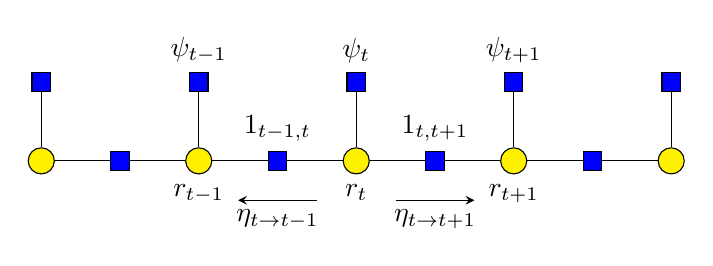
\begin{tikzpicture}[>=stealth]
        \node[circle, draw, fill=yellow] (A) at (0,0) {};
        \node[rectangle, draw, fill=blue] (B) at (1,0) {};
        \node[circle, draw, fill=yellow, label=below:\( r_{t-1} \)] (C) at (2,0) {};
        \node[rectangle, draw, fill=blue, label=above:\( \mathbbm{1}_{t-1, t} \)] (D) at (3,0) {};
        \node[circle, draw, fill=yellow, label=below:\( r_{t} \)] (E) at (4,0) {};
        \node[rectangle, draw, fill=blue, label=above:\( \mathbbm{1}_{t, t+1} \)] (F) at (5,0) {};
        \node[circle, draw, fill=yellow, label=below:\( r_{t+1} \)] (G) at (6,0) {};
        \node[rectangle, draw, fill=blue] (H) at (7,0) {};
        \node[circle, draw, fill=yellow] (I) at (8,0) {};
        \node[rectangle, draw, fill=blue] (J) at (0,1) {};
        \node[rectangle, draw, fill=blue, label=above:\( \psi_{t-1} \)] (K) at (2,1) {};
        \node[rectangle, draw, fill=blue, label=above:\( \psi_{t} \)] (L) at (4,1) {};
        \node[rectangle, draw, fill=blue, label=above:\( \psi_{t+1} \)] (M) at (6,1) {};
        \node[rectangle, draw, fill=blue] (N) at (8,1) {};

        \draw[-] (A) -- (B);
        \draw[-] (B) -- (C);
        \draw[-] (C) -- (D);
        \draw[-] (D) -- (E);
        \draw[-] (E) -- (F);
        \draw[-] (F) -- (G);
        \draw[-] (G) -- (H);
        \draw[-] (H) -- (I);
        \draw[-] (A) -- (J);
        \draw[-] (C) -- (K);
        \draw[-] (E) -- (L);
        \draw[-] (G) -- (M);
        \draw[-] (I) -- (N);

        \draw[->] (4.5,-0.5) -- (5.5,-0.5) node[midway, below] {\( \eta_{t \to t+1} \)};
        \draw[<-] (2.5,-0.5) -- (3.5,-0.5) node[midway, below] {\( \eta_{t \to t-1} \)};
    \end{tikzpicture}
    \caption[
        شبکه برهمکنش متغیرهای
        \( r_{t} \)
        و قیدهای حاکم بر این متغیر‌ها
    ]
    {
        شبکه برهمکنش متغیرهای
        \( r_{t} \)
        و قیدهای حاکم بر این متغیر‌ها. گره‌های دایره‌ای زرد نشان‌دهنده گره‌های متغیر و گره‌های مربعی آبی نشان‌دهنده گره‌های قیدی حاکم بر متغیرهای
        \( r_{t} \)
        است.
    }
    \label{fig:factor_graph}
\end{figure}

همان‌طور که در
\autoref{fig:factor_graph}
مشاهده می‌کنید، می‌توان
\autoref{eq:probability_product}
را به شکل شبکه‌ای از برهمکنش‌های بین اجزای سیستم نمایش داد.
این شبکه شامل گره‌های متغیر
\( r_{t} \)
است که با دایره‌های زرد مشخص شده‌اند
و گره‌های قیدی
\( \psi_{t}(r_{t}) \) و \( \mathbbm{1}(r_{t}, r_{t+1}) \)
مربع‌های آبی هستند که محدودیت‌های دینامیکی و احتمالاتی را بر روی گره‌های متغیر اعمال می‌کنند.

نمایش تابع احتمال
\( P(\mathbf{r}) \)
به شکل بالا، نشان‌دهنده‌ی کارکرد مناسب تقریب بته در تحلیل و بررسی تعداد جواب‌های دینامیکی این سیستم است.
با استفاده از این تقریب، می‌توان احتمال رخداد حالت
\( r_{t} \)
در هر گره را به صورت ضرب احتمال حالت‌های همسایه‌های آن گره بیان کرد.
در نتیجه، می‌توان معادله‌های زیر را برای تابع توزیع احتمال حاشیه‌ای هر متغیر نوشت.

تابع توزیع احتمال حاشیه‌ای برای متغیر
\( r_{t} \)
در غیاب برهمکنش بین گره‌های
\( r_{t} \) و \( r_{t+1} \)
به شکل زیر بیان می‌شود:
\begin{equation} \label{eq:bp_constraint}
    \eta_{t \to t+1}(r_{t}) = \frac{\psi_{t}(r_{t})}{z_{t \to t+1}} \sum_{r_{t-1}} \eta_{t-1 \to t}(r_{t-1}) \mathbbm{1}(r_{t-1},r_{t})
\end{equation}
این معادله نشان می‌دهد که توزیع احتمال حاشیه‌ای برای متغیر
\( r_{t} \)
هنگامی که متغیر
\( r_{t+1} \)
و تمام همسایه‌های آن به جز متغیر
\( r_{t} \)
از شبکه‌ی برهمکنش‌ها حذف شده باشند را
می‌توان به صورت ضرب احتمال رخداد حالت
\( r_{t} \)،
یعنی
\( \psi(r_{t}) \)
که از تابع توزیع بولتزمن پیروی می‌کند و
احتمال‌های حاشیه‌ای مربوط به همسایه‌های
\( r_{t} \)، یعنی
\( \eta_{t-1 \to t}(r_{t-1}) \)
و قید‌های دینامیکی مدل دینامیکی، یعنی
\( \mathbbm{1}(r_{t-1},r_{t}) \)،
بیان کرد.

با توجه به رابطه بالا، می‌توان
توزیع احتمال حاشیه‌ای برای متغیر
\( r_{t} \)
با در نظر گرفتن همه‌ی همسایه‌ها
به شکل زیر بیان کرد:
\begin{equation} \label{eq:bp_variable}
    \eta_{t}(r_{t}) = \frac{\psi_{t}(r_{t})}{z_{t}} \left( \sum_{r_{t-1}} \eta_{t-1 \to t}(r_{t-1}) \mathbbm{1}(r_{t-1},r_{t}) \right) \left( \sum_{r_{t+1}} \eta_{t+1 \to t}(r_{t+1}) \mathbbm{1}(r_{t},r_{t+1}) \right)
\end{equation}

همچنین، ثابت‌های بهنجارش
\( z_{t \to t+1} \) و \( z_{t} \)
که در معادله‌های
\ref{eq:bp_constraint} و \ref{eq:bp_variable}
آمده‌اند، به صورت زیر تعریف می‌شوند:
\begin{equation} \label{eq:bp_normalization_constraint}
    z_{t \to t+1} = \sum_{r_{t}} \psi_{t}(r_{t}) \sum_{r_{t-1}} \eta_{t-1 \to t} \mathbbm{1}(r_{t-1},r_{t})
\end{equation}
\begin{equation} \label{eq:bp_normalization_variable}
    z_{t} = \sum_{r_{t}} \psi_{t}(r_{t}) \left( \sum_{r_{t-1}} \eta_{t-1 \to t}(r_{t-1}) \mathbbm{1}(r_{t-1},r_{t}) \right) \left( \sum_{r_{t+1}} \eta_{t+1 \to t}(r_{t+1}) \mathbbm{1}(r_{t},r_{t+1}) \right)
\end{equation}

تابع توزیع‌های احتمال حاشیه‌ای که توسط معادله‌های
\ref{eq:bp_constraint} و \ref{eq:bp_variable}
توصیف می‌شوند را می‌توان به شکل پیام‌هایی تعبیر کرد که بین متغیرها رد و بدل می‌شوند.
به همین دلیل، این معادله‌ها به نام معادله‌های انتشار باور نیز شناخته می‌شوند.
حالت کلی این معادله‌ها و روش به دست آوردن آن‌ها در
\ref{app:belief_propagation}
آمده است.
\cite{yedidia2005,mezard2009,zdeborova2016}.

با دانستن توزیع‌های احتمال حاشیه‌ای می‌توان چگالی آنتروپی آزاد و در نتیجه میانگین انرژی و آنتروپی سیستم را محاسبه کرد.
برای این منظور، یعنی یافتن جواب‌های تابع توزیع‌های احتمال حاشیه‌ای، می‌توان از الگوریتم انتشار باور استفاده کرد.
در زیر شبه کد این الگوریتم آورده شده است
\cite{zdeborova2016}.
\begin{algorithm}[H]
    \caption{الگوریتم انتشار باور}
    \begin{algorithmic}[1]
        \STATE \( \eta_{t \to t+1}(r_{t}) \)
        را با مقدار‌هایی تصادفی مقداردهی کنید.
        \STATE \( \eta_{t \to t+1}(r_{t}) \)
        را با استفاده از
        \autoref{eq:bp_constraint}
        به‌روزرسانی کنید.
        \STATE گام ۲ را تا همگرا شدن
        \( \eta_{t \to t+1}(r_{t}) \)
        به یک مقدار ثابت تکرار کنید.
        \STATE \( \eta_{t}(r_{t}) \)
        را محاسبه کنید.
    \end{algorithmic}
\end{algorithm}

پس از به دست آوردن احتمال‌های حاشیه‌ای، می‌توان از آن‌ها برای محاسبه‌ی چگالی آنتروپی آزاد استفاده کرد.
چگالی آنتروپی آزاد محاسبه شده از احتمال‌های حاشیه‌ای، به عنوان آنتروپی آزاد بته شناخته می‌شود و به صورت زیر محاسبه می‌شود:
\begin{equation} \label{eq:bethe_free_energy}
    \Phi = \frac{1}{\mathcal{\mathcal{T}}} \ln Z = \frac{1}{\mathcal{\mathcal{T}}} \left( \sum_{t=1}^{\mathcal{\mathcal{T}}} \ln z_{t} - \sum_{t=1}^{\mathcal{\mathcal{T}}-1} \ln z_{t,t+1} \right)
\end{equation}
در اینجا،
\( z_{t} \)
سهم متغیر
\( r_{t} \)
در تابع پارش است که تغییر در تابع پارش را هنگام اضافه شدن متغیر
\( r_{t} \)
و برهمکنش‌های مرتبط با آن به سیستم توصیف می‌کند و توسط
\autoref{eq:bp_normalization_variable}
داده می‌شود.
همچنین،
\( z_{t,t+1} \)
سهم برهمکنش‌های بین متغیرهای
\( r_{t} \) و \( r_{t+1} \)
است و تغییر در تابع پارش را هنگام اضافه شدن این برهمکنش‌ها به سیستم توصیف می‌کند.
این مقدار به صورت زیر به دست می‌آید:
\begin{equation} \label{eq:partial_partition_function}
    z_{t,t+1} = \sum_{r_{t}} \sum_{r_{t+1}} \eta_{t \to t+1}(r_{t}) \eta_{t+1 \to t}(r_{t+1}) \mathbbm{1}(r_{t},r_{t+1})
\end{equation}
در این معادله
\( \eta_{t \to t+1}(r_{t}) \) و \( \eta_{t+1 \to t}(r_{t+1}) \)
جواب‌های
\autoref{eq:bp_constraint}
هستند.

\autoref{eq:bethe_free_energy}
در واقع مجموع آنتروپی آزاد همه‌ی متغیرها را توصیف می‌کند.
اما از آنجا که در این مجموع هر برهمکنش دو بار شمارش می‌شود، برای تصحیح این شمارش اضافی، آنتروپی آزاد مربوط به برهمکنش‌ها از مجموع کسر می‌شود.
\cite{mezard2003}.

با این حال، حل معادله‌های انتشار باور و یافتن جواب‌های این معادله‌ها در اینجا به صورت تحلیلی ممکن نیست.
علاوه بر این، محاسبه‌ی عددی جواب‌های معادله‌های انتشار باور به دلیل پیوسته بودن فضای
\( r \)
دشوار است و نیاز به گسسته‌سازی فضای
\( r \)
دارد که این باعث افزایش حجم محاسبات می‌شود.
در نتیجه، استفاده از روش های عددی دیگر، نظیر روش دینامیک جمعیت\LTRfootnote{Population dynamics} به عنوان روشی مناسب برای حل این مسئله و یافتن جواب‌های معادله‌های انتشار باور به صورت تقریبی پیشنهاد می‌شود
\cite{mezard2001}.

روش دینامیک جمعیت به این صورت عمل می‌کند که توزیع‌های احتمال حاشیه‌ای را به شکل جمعیتی از مقدار‌های
\( r_{i} \)
در نظر می‌گیرد.
این جمعیت‌ها از طریق به‌روزرسانی بر اساس دینامیک سیستم موردنظر ما، یعنی نگاشت چیالوو و مقایسه انرژی آن‌ها، به سمت جواب‌های پایای توزیع‌های احتمال حاشیه‌ای هدایت می‌شوند.
در نهایت، با استفاده از این جمعیت‌ها، آنتروپی آزاد و آنتروپی سیستم محاسبه می‌شود.
شبه کد الگوریتم دینامیک جمعیت را به شکل زیر آورده شده است:
\begin{algorithm}[H]
    \caption{الگوریتم دینامیک جمعیت}
    \begin{algorithmic}[1]
        \STATE \( \eta_{t \to t+1} \)
        را با مقدار‌هایی تصادفی مقداردهی کنید.
        \STATE به صورت تصادفی
        \( r_{i} \)
        را از جمعیت
        \( \eta_{t-1 \to t} \) و \( r_{j} \)
        را از جمعیت
        \( \eta_{t \to t+1} \)
        انتخاب کنید.
        \STATE مقدار
        \( r_{\text{new}} = f(r_{i}) \)
        را محاسبه کرده و انرژی آن،
        \( E(r_{\text{new}}) \)،
        را تعیین کنید.
        \STATE اگر
        \( E(r_{\text{new}}) < E(r_{j}) \)
        شد،
        \( r_{\text{new}} \)
        را جایگزین
        \( r_{j} \)
        در جمعیت
        \( \eta_{t \to t+1} \)
        کنید.
        \STATE اگر
        \( E(r_{\text{new}}) > E(r_{j}) \)
        شد، با احتمال
        \( e^{-\beta \Delta E} \)، \( r_{\text{new}} \)
        را جایگزین
        \( r_{j} \)
        در جمعیت
        \( \eta_{t \to t+1} \)
        کنید.
        \STATE گام‌های ۲ تا ۵ را تا همگرا شدن جمعیت‌
        \( \eta_{t \to t+1} \)
        به یک مقدار ثابت تکرار کنید.
        \STATE گام‌های ۱ تا ۶ را برای
        \( \eta_{t \to t-1} \)
        نیز تکرار کنید.
    \end{algorithmic}
\end{algorithm}

برای یافتن تعداد جواب‌های دینامیکی مسئله و همچنین برای محاسبه‌ی میانگین فاصله‌ها از دنباله مرجع، از الگوریتم انتشار باور و روش دینامیک جمعیت استفاده کردیم.
این شبیه‌سازی‌ها را برای محاسبه‌ی انرژی و آنتروپی دنباله‌های مشاهده شده از نگاشت چیالوو بر اساس دنباله مرجع مشخصی انجام دادیم.
در این شبیه‌سازی‌ها، تنها تفاوت در شرایط اولیه‌ی دنباله‌های مشاهده شده، یعنی
\( r_{0} = (x_{0}, y_{0}) \)
بوده است، در حالی که پارامترهای نگاشت چیالوو برای دو ناحیه زیر ثابت نگه داشته شده‌اند:
\begin{itemize}[label=-]
    \item مرز بین ناحیه غیربرانگیخته و برانگیخته با پارامتر‌های
          \( a = 0.89 \)، \( b = 0.60 \)، \( c = 0.28 \) و \( k = 0.030 \)
    \item مرز بین ناحیه غیربرانگیخته و آشوبناک با پارامترهای
          \( a = 0.89 \)، \( b = 0.18 \)، \( c = 0.28 \) و \( k = 0.023 \)
\end{itemize}
در این شبیه‌سازی‌ها، پارامتر
\( \beta \)
در بازه‌ای مشخص تغییر دادیم تا میانگین انرژی و آنتروپی سیستم برای دنباله‌هایی با طول‌های ۳ و ۶ محاسبه کنیم.
نتایج به دست آمده برای میانگین انرژی و آنتروپی این سیستم به شرح زیر نمایش داده شده‌اند:
\begin{itemize}[label=-]
    \item برای دنباله‌های با طول ۳، نتایج در
          \autoref{fig:bp_3}
          نمایش داده شده‌اند.
    \item برای دنباله‌های با طول ۶، نتایج در
          \autoref{fig:bp_6}
          نمایش داده شده‌اند.
\end{itemize}

\begin{figure}
    \centering
    \includegraphics[height=0.9\textheight]{figures/bp_3}
    \caption{
        رفتار میانگین انرژی و آنتروپی نسبت به تغییر پارامتر
        \( \beta \)
        برای دنباله‌هایی با طول ۳
    }
    \label{fig:bp_3}
\end{figure}

همان‌طور که در
\autoref{fig:bp_3}
مشاهده می‌کنید، رفتار آنتروپی برای دنباله‌های با طول ۳ به گونه‌ای است که مقدار آنتروپی و تعداد جواب‌های دینامیکی در هر دو ناحیه‌ی مرز ناحیه برانگیخته و مرز ناحیه آشوبناک به خوبی از هم متمایز شده‌اند.
در این شکل می‌بینیم که تعداد جواب‌های دینامیکی در مرز ناحیه برانگیخته کمتر از مرز ناحیه آشوبناک است.
همچنین، با افزایش پارامتر
\( \beta \)،
تعداد جواب‌های دینامیکی در مرز ناحیه برانگیخته با شیب بیشتری نسبت به مرز ناحیه آشوبناک کاهش می‌یابند.
علاوه بر این، یک رفتار غیرمتعارف در آنتروپی نسبت به افزایش مقدار
\( \beta \)
و کاهش انرژی مشاهده می‌شود که در ادامه به تحلیل دقیق‌تر آن خواهیم پرداخت.

\begin{figure}
    \centering
    \includegraphics[height=0.9\textheight]{figures/bp_6}
    \caption{
        رفتار میانگین انرژی و آنتروپی نسبت به تغییر پارامتر
        \( \beta \)
        برای دنباله‌هایی با طول ۶
    }
    \label{fig:bp_6}
\end{figure}

در
\autoref{fig:bp_6}
رفتار میانگین انرژی و آنتروپی را برای دنباله‌هایی با طول ۶ مشاهده می‌کنید.
رفتار میانگین انرژی و آنتروپی در این طول نیز مشابه رفتار آن‌ها در طول ۳ است.
با این حال، با افزایش طول دنباله‌ی مشاهده شده، تعداد جواب‌های دینامیکی یا همان آنتروپی برای تمام مقدارهای
\( \beta \)
افزایش یافته است.
همچنین، رفتار غیرمتعارفی که در طول ۳ مشاهده می‌شد، در اینجا مشاهده نمی‌شود.

همان‌طور که گفته شد، در رفتار آنتروپی برای دنباله‌های با طول ۳،
\autoref{fig:bp_3}،
یک روند غیرمتعارف نسبت به پارامتر
\( \beta \)
و میانگین انرژی مشاهده می‌شود.
به این صورت که با افزایش
\( \beta \)
و کاهش انرژی، آنتروپی ابتدا افزایش یافته و سپس کاهش می‌یابد.
در حالی که انتظار می‌رود با کاهش انرژی، آنتروپی به طور یکنواخت کاهش یابد اما این رفتار در نتایج مشاهده نمی‌شود.

این رفتار غیرمتعارف ناشی از نحوه‌ی گسسته‌سازی پارامتر‌ها برای انجام شبیه‌سازی‌های عددی است.
می‌توان این رفتار را این گونه توضیح داد که در جایی که فاصله‌ی دنباله‌های مشاهده شده از دنباله مرجع زیاد است، با کاهش فاصله‌ی دنباله‌ها و میانگین انرژی، تعداد حالت‌هایی که قیدهای موجود در محاسبات عددی را برآورده می‌کنند، افزایش می‌یابند.
این افزایش در تعداد حالت‌های پذیرفته شده باعث افزایش آنتروپی و تعداد جواب‌های دینامیکی می‌شود.
با ادامه‌ی کاهش فاصله و میانگین انرژی، تعداد این حالت‌ها که تنها به دلیل قید‌های محاسبات عددی در سیستم وارد شده‌اند کاهش می‌یابند و رفتار آنتروپی به حالت مورد انتظار باز می‌گردد و کاهش می‌یابد.

\begin{figure}[!ht]
    \centering
    \includegraphics[width=0.8\textwidth]{figures/artifact}
    \caption{مقایسه رفتار غیرمتعارف آنتروپی برای دو نحوه‌ی متفاوت در گسسته‌سازی پارامترها}
    \label{fig:artifact}
\end{figure}

در
\autoref{fig:artifact}
این رفتار غیرمتعارف برای دو شبیه‌سازی با گسسته‌سازی‌های مختلف نشان داده شده است.
همان‌طور که مشاهده می‌کنید، با تغییر در نحوه‌ی گسسته‌سازی در محاسبه‌های عددی، این رفتار غیرمتعارف در آنتروپی بیشتر نمایان می‌شود.
به طوری که با افزایش تعداد نقاط گسسته‌سازی، مقدار آنتروپی در بازه‌ی بزرگ‌تری افزایش یافته است.
بنابراین، در شبیه‌سازی‌های بعدی باید این نکته را در نظر گرفت و پارامتر‌ها را به طور مناسب گسسته کرد.

\section{تصحیح خطا با روش مونته‌کارلو}
فرض کنید دنباله مرجع
\( \mathbf{r}^{*} \)
از یک نورون سالم مشاهده شده است.
نورون‌هایی بیمار وجود دارند که به دلیل خطا در پارامترهای خود، دنباله
\( \mathbf{r} \)
را تولید می‌کنند.
هدف ما این است که با تنظیم مناسب پارامترها، فاصله بین دنباله‌ی مرجع و دنباله‌ی مشاهده شده از نورون بیمار را کمینه کنیم.
یکی از روش‌های مناسب برای تصحیح این خطا و کمینه کردن فاصله بین دنباله‌ها، استفاده از روش مونته‌کارلو است.

معرفی و استفاده از روش‌های مونته‌کارلو به مقاله‌ی معروف متروپلیس و همکاران
\cite{metropolis1953}
بازمی‌گردد.
الگوریتم متروپلیس-هستینگز
\cite{metropolis1953,hastings1970}
بر اساس مقایسه‌ی هزینه‌ی اختلاف انرژی بین یک حالت از سیستم و همان حالت پس از ایجاد یک تغییر کوچک در آن حالت است.
اگر این تغییر باعث کاهش هزینه شود، پذیرفته می‌شود اما اگر هزینه افزایش یابد، تغییر با احتمالی متناسب با اختلاف هزینه پذیرفته خواهد شد.
این فرآیند با ایجاد تغییرهای کوچک، به طور پیوسته ادامه می‌یابد تا انرژی سیستم به یک مقدار کمینه برسد
\cite{newman1999,landau2021}.

یکی از مزیت‌های مهم روش‌های مبتنی بر مونته‌کارلو این است که اگر برای مدت زمان کافی، تغییر در حالت سیستم تکرار شود، می‌توانند پاسخی دقیق را برای یک کلاس بسیار عمومی و گسترده از سیستم‌ها ارائه دهند.
با این حال، نقطه ضعف این روش‌ها در این است که زمان لازم برای به دست آوردن نتیجه‌ی دقیق می‌تواند با افزایش اندازه‌ی سیستم به صورت نمایی افزایش یابد.
به همین دلیل، تصمیم‌گیری در مورد زمان لازم برای رسیدن به دقت مطلوب بسیار دشوار است
\cite{zdeborova2016}.
با این وجود، استفاده از این روش می‌تواند دیدگاه مناسبی را نسبت به رفتار خطا در مدل نورونی مورد مطالعه‌ی ما، یعنی نگاشت چیالوو، فراهم کند.

برای تصحیح خطا در پارامترهای این مدل نورونی، مراحل زیر را دنبال می‌کنیم.
ابتدا فرض می‌کنیم که پارامترهای نورون سالم
\( \theta^{*} \)
متناسب با پارامتر
\( \varepsilon \)
به شکل زیر دچار خطا شده‌اند:
\[ \theta = (1 + \varepsilon) \theta^{*} \]
که در اینجا
\( -1 < \varepsilon < 1 \)
است.
در ادامه، برای کاهش فاصله‌ی بین دنباله‌ی مرجع و دنباله‌ی مشاهده شده از نورون بیمار، از روش مونته‌کارلو استفاده می‌کنیم.
به این ترتیب که در هر گام، پارامتر
\( \theta \)
را به اندازه یک مقدار تصادفی
\( \delta \)
در بازه‌ی مناسب آن پارامتر به شکل زیر تغییر می‌دهیم:
\[ \theta_{\text{new}} = (1 + \delta) \theta \]
سپس فاصله‌ی بین دنباله‌ی دینامیکی حاصل از پارامتر
\( \theta_{\text{new}} \)
و دنباله‌ی نورون سالم را محاسبه می‌کنیم.
در صورتی که این فاصله، کاهش یافته بود، پارامتر
\( \theta_{\text{new}} \)
را به عنوان پارامتر جدید سیستم در نظر می‌گیریم.
این فرآیند را تا زمانی که فاصله به یک مقدار حداقلی مطلوب برسد یا تعداد گام‌های مونته‌کارلو به یک مقدار حداکثری برسد، تکرار می‌کنیم.

پس از یافتن کمینه فاصله‌ی بین دنباله‌های نورون بیمار و نورون سالم، خطای پارامترها را با استفاده از رابطه‌ی زیر محاسبه می‌کنیم:
\begin{equation}
    \Delta \theta = \left[ \left( 1 - \frac{a}{a^{*}} \right)^2 + \left( 1 - \frac{b}{b^{*}} \right)^2 + \left( 1 - \frac{c}{c^{*}} \right)^2 + \left( 1- \frac{k }{k^{*}} \right)^2 \right]^{\frac{1}{2}}
\end{equation}
در اینجا
\( a^{*} \)، \( b^{*} \)، \( c^{*} \) و \( k^{*} \)
پارامترهای نورون سالم و
\( a \)، \( b \)، \( c \) و \( k \)
پارامترهای نهایی به دست آمده از روش مونته‌کارلو هستند.
با تکرار روش مونته‌کارلو برای مقدارهای مختلف
\( \varepsilon \)
و همچنین شرایط اولیه‌ی متفاوت برای دنباله‌ها،
\( r_{0} \)،
آنسامبلی از خطاهای پارامترها به دست می‌آید.

برای تحلیل رفتار خطای پارامتر‌های یک مدل نورونی، با توجه به طول دنباله‌ی مشاهده شده و مقدار خطای اولیه
\( \varepsilon \)،
شبیه‌سازی‌هایی را با روشی که در بالا توضیح داده شد، انجام دادیم.
این شبیه‌سازی‌ها برای دو ناحیه‌ی مختلف از فضای پارامتری یک نورون انجام شده‌اند:
\begin{itemize}[label=-]
    \item مرز بین ناحیه غیربرانگیخته و برانگیخته با پارامتر‌های
          \( a = 0.89 \)، \( b = 0.60 \)، \( c = 0.28 \) و \( k = 0.030 \)
    \item مرز بین ناحیه غیربرانگیخته و آشوبناک با پارامترهای
          \( a = 0.89 \)، \( b = 0.18 \)، \( c = 0.28 \) و \( k = 0.023 \)
\end{itemize}
نتایج این شبیه‌سازی‌ها برای این دو ناحیه به شرح زیر است:

\subsubsection{مرز بین ناحیه غیربرانگیخته و برانگیخته}

\begin{figure}[!ht]
    \centering
    \includegraphics[width=0.9\textwidth]{figures/error_excitable}
    \caption{رفتار خطای نسبی پارامترها در مرز ناحیه غیربرانگیخته و برانگیخته}
    \label{fig:error_excitable}
\end{figure}

همان‌طور که در
\autoref{fig:error_excitable}
مشاهده می‌کنید، با افزایش طول دنباله‌ی مشاهده شده از یک نورون بیمار، مقدار کمینه خطای پارامترها ابتدا به سرعت کاهش یافته و سپس
برای دنباله‌های با طول بیشتر از ۶، در یک بازه نسبتاً طولانی تقریباً ثابت باقی می‌ماند.
این به این معنی است که دنباله‌های با طول بیشتر از ۶ اطلاعات بیشتری از رفتار نورون فراهم نمی‌کنند.
در نتیجه، برای کمینه کردن و تصحیح خطای پارامترها، مشاهده دنباله‌هایی به طول ۶ از دینامیک نورون کافی است.

این طول مشخصه، ممکن است به دو عامل وابسته باشد.
اولین عامل می‌تواند مدت زمان لازم برای گذار نورون به حالت پایدار خود پس از ایجاد خطا در پارامتر‌های مدل باشد.
دومین عامل نیز می‌تواند به مدت زمان یک اسپایک بستگی داشته باشد، زیرا عمده اطلاعات مربوط به دینامیک یک سیستم نورونی در رفتار پتانسیل عمل آن نورون نهفته است.

\subsubsection{مرز بین ناحیه غیربرانگیخته و آشوبناک}

\begin{figure}[!ht]
    \centering
    \includegraphics[width=0.9\textwidth]{figures/error_chaotic}
    \caption{رفتار خطای نسبی پارامترها در مرز ناحیه غیربرانگیخته و آشوبناک}
    \label{fig:error_chaotic}
\end{figure}

همان‌طور که در
\autoref{fig:error_chaotic}
مشاهده می‌کنید،
رفتار کمینه خطای پارامترها در این ناحیه با رفتار کمینه خطا در مرز ناحیه برانگیخته متفاوت است.
در اینجا، کمینه خطای پارامترها در ابتدا با افزایش طول دنباله مشاهده شده با شیب بسیار کمتری نسبت به مرز ناحیه برانگیخته کاهش می‌یابد، اما پس از آن و با افزایش بیشتر طول دنباله، خطا افزایش می‌یابد.
این رفتار را می‌توان این چنین توضیح داد که در دنباله‌های کوتاه‌تر، افزایش طول دنباله مشاهده شده اطلاعات بیشتری از رفتار سیستم فراهم می‌کند.
در نتیجه، در ابتدا کاهش خطای پارامترها با افزایش طول دنباله مشاهده شده آسان‌تر است.
اما با افزایش بیشتر طول دنباله مشاهده شده، به دلیل ماهیت آشوبناک سیستم و دور شدن دنباله‌ها به صورت نمایی از یکدیگر، یافتن پارامترهای مناسب دشوارتر شده و مقدار کمینه خطا افزایش می‌یابد.

در این ناحیه، مشاهده دیگری که قابل توجه است، وابستگی طول دنباله‌ی لازم برای رسیدن به کمینه خطا به مقدار اولیه خطای پارامترها است.
به طوری که هر چه خطای اولیه بیشتر باشد، دنباله‌هایی با طول بلندتر برای رسیدن به کمینه خطا نیاز است.
همچنین، مقدار کمینه خطا نیز به خطای اولیه بستگی دارد و هر چه خطای اولیه بزرگتر باشد، مقدار کمینه خطا نیز بزرگتر خواهد بود.

\chapter{جمع‌بندی و پیشنهادها} \label{chap:discussion}

\section{جمع‌بندی}
نورون‌ها و به تبع آن سیستم عصبی، همواره در معرض بیماری‌ها قرار دارند.
بیماری در یک نورون را می‌توان به صورت اختلالی در پارامترهای مدل دینامیکی آن نورون در نظر گرفت.
این اختلال در پارامترهای مدل دینامیکی منجر به تولید دنباله‌ی دینامیکی متفاوت از دینامیک یک نورون سالم خواهد شد.
برای مشخصه‌یابی اثر این خطاها در مدل، تعداد جواب‌های معادله دینامیکی را که فاصله مشخصی از دنباله‌ی نورون سالم دارند، معین کردیم.
نتایج نشان می‌دهند که با کاهش فاصله از دنباله مربوط به نورون سالم، تعداد جواب‌ها کاهش می‌یابد و این کاهش در مرز ناحیه‌ی برانگیخته نسبت به مرز ناحیه‌ی آشوبناک محسوس‌تر است.
همچنین، در این پژوهش، با استفاده از روش مونته‌کارلو به تصحیح و کاهش خطاهای پارامترها در مدلی از یک نورون پرداختیم.
نتایج نشان می‌دهند که در مرز ناحیه‌ی برانگیخته، با افزایش طول دنباله‌ی مشاهده شده، خطاهای پارامترها به سرعت کاهش یافته و پس از رسیدن به مقداری مشخص، در دنباله‌های بلندتر تقریباً ثابت می‌مانند.
این رفتار یک طول مشخصه را فراهم می‌کند که می‌تواند برای تصحیح خطا بسیار مهم باشد.
به طوری که برای کاهش خطا در مرز ناحیه برانگیخته تنها به دنباله‌هایی با این طول مشخصه نیاز است و نیازی به داشتن دنباله‌های بلندتر ضروری نیست.
در مرز ناحیه‌ی آشوبناک، رفتاری متفاوت مشاهده می‌شود.
به این گونه که با افزایش طول دنباله، خطای پارامترها کاهش می‌یابد.
اما پس از مدتی روندی افزایشی پیدا می‌کند.
علاوه بر این، طول دنباله‌ای که به کمینه خطا منجر می‌شود با مقدار اولیه خطای پارامترها متناسب است، به طوری که خطای اولیه بیشتر، به دنباله‌ای با طول بلندتر برای رسیدن به مقدار کمینه نیاز دارد.

\section{پیشنهادها}
در این پژوهش، به بررسی خطاهای پارامتری در یک مدل دینامیکی از تک نورون پرداختیم.
با این حال، اختلا‌ل‌ها و بیماری‌ها نه تنها در سطح یک نورون، بلکه در ارتباطات بین نورون‌ها و در نهایت در شبکه‌ای از نورون‌ها نیز رخ می‌دهند.
بنابراین، تعمیم این بررسی‌ها به شبکه‌های نورونی می‌تواند گام بعدی این تحقیق باشد.
در این مطالعه، از الگوریتم مونته‌کارلو برای تصحیح خطاها استفاده شد.
به کارگیری الگوریتم‌های بهینه‌تر و دقیق‌تر می‌تواند به عنوان گام بعدی مطرح باشد.
همچنین، در بخش تشخیص خطا، تنها تأثیر شرایط اولیه بر فاصله دنباله‌ها بررسی شد.
در آینده می‌توان تأثیر خطای پارامترها را نیز بر این فاصله مطالعه کرد تا درک عمیق‌تری از تأثیر این خطاها بر رفتار کلی سیستم به دست آید.
علاوه بر این، در این پژوهش، تنها به بررسی رفتار خطاها در مرز بین ناحیه‌ی غیربرانگیخته و برانگیخته و مرز بین ناحیه‌ی غیربرانگیخته و آشوبناک پرداختیم.
در آینده، بررسی رفتار خطا در مرز ناحیه‌ی برانگیخته و آشوبناک که در علوم اعصاب بسیار مهم است نیز باید مدنظر قرار گیرد.


\pagestyle{plain}

\begin{latin}
    \singlespacing
    \printbibliography
\end{latin}
\thispagestyle{empty}
\addappheadtotoc
\centerline{\textbf{\appendixtocname}}

\begin{appendices}
    \app{انتشار باور} \label{app:belief_propagation}
    در یک سیستم آماری، تعداد حالت‌هایی که انرژی معینی دارند با
    \( \mathcal{N}(E) \)
    نشان داده می‌شود و آنتروپی
    \( S(E) \)
    را بر اساس آن به صورت زیر تعریف می‌شود:
    \begin{equation} \label{eq:number_density}
        \mathcal{N} (E) = e^{N S(E)}
    \end{equation}
    که در آن
    \( E \)
    چگالی انرژی و
    \( S \)
    چگالی آنتروپی است.
    اگر
    \( \Phi(\beta) \)
    را به عنوان چگالی آنتروپی آزاد در نظر بگیریم، می‌توان تابع پارش سیستم را به صورت زیر بازنویسی کرد:
    \begin{equation} \label{eq:partition_function}
        e^{N \Phi(\beta)} = Z = \sum_{\{ s_{i} \}_{i=1}^{N}} e^{-\beta E} = \sum_{E} \sum_{\text{\lr{All states with energy}} E} e^{-N \beta E} = \int dE \, e^{N (S(E) - \beta E)}
    \end{equation}
    در اینجا، جمع روی همه حالت‌ها به جمع روی حالت‌های با انرژی
    \( E \)
    و جمع روی تمام مقادیر مخلتف انرژی تجزیه شده است.
    همچنین، با استفاده از
    \autoref{eq:number_density}
    جمع روی تمام حالت‌ها با انرژی
    \( E \)
    را با تعداد این حالت‌ها جایگزین کرده و سپس جمع روی مقادیر گسسته
    \( E \)
    را به انتگرال تبدیل کرده‌ایم.

    با توجه به
    \autoref{eq:partition_function}
    و در نظر گرفتن حد
    \( N \to \infty \)
    و استفاده از روش نقطه زینی، روابط زیر به دست می‌آیند:
    \begin{equation}
        \left. \frac{\partial S(E)}{\partial E} \right|_{E = E^{*}} = \beta, \qquad \Phi(\beta) = S(E^{*}) - \beta E^{*}
    \end{equation}
    در دمای
    \( \beta \)
    از یک حالت تصادفی
    نمونه‌برداری شود، انرژی آن در
    \( E^{*} = \langle E \rangle \)
    متمرکز است.
    این به این معنی است که توزیع بولتزمن انتخاب مناسبی برای احتمال رخداد یک حالت انرژی معین است، زیرا:
    \begin{equation}
        \frac{d \Phi(\beta)}{d \beta} = - \langle E \rangle
    \end{equation}

    اگر بتوان چگالی آنتروپی آزاد
    \( \Phi \)
    را به عنوان تابعی از
    \( \beta \)
    محاسبه کرد، می‌توان با محاسبه‌ی مشتق‌های آن، میانگین انرژی و تعداد حالت‌ها با یک انرژی معین
    \( S(E) \)
    را به دست آورد.
    این محاسبات معمولاً پیچیده و به لحاظ محاسباتی دشوار است.
    بنابراین، برای به دست آوردن نتایج تقریبی و در برخی موارد دقیق، می‌توان از الگوریتم انتشار باور و آنتروپی آزاد بته استفاده کرد.

    حال تابع توزیع احتمال زیر را در نظر بگیرید:
    \begin{equation} \label{eq:probability_distribution}
        P \left( \{ s_{i} \}_{i=1}^{N} \right) = \frac{1}{Z} \prod_{i=1}^{N} g_{i}(s_{i}) \prod_{a=1}^{M} f_{a}(\{ s_{i} \}_{i \in \partial a})
    \end{equation}
    این تابع توزیع بیان می‌کند که احتمال رخداد حالت
    \( \{ s_{i} \}_{i=1}^{N} \)
    متناسب با احتمال رخداد هر حالت
    \( g_{i}(s_{i}) \)
    و قیدهای
    \( f_{a}(\{ s_{i} \}_{i \in \partial a}) \)
    است که نشان دهنده‌ی برهمکنش‌های سیستم است.
    در اینجا، تعداد متغیرها
    \( N \)
    است و مجموعه‌ای از
    \( M \)
    قید در سیستم وجود دارد.

    همان‌طور که می‌دانیم، کمیت‌های مورد علاقه را می‌توان از ثابت بهنجارش
    \autoref{eq:probability_distribution}
    یا همان تابع پارش استخراج کرد:
    \begin{equation}
        Z = \sum_{\{ s_{i} \}_{i=1}^{N}} \prod_{i}^{N} g_{i}(s_{i}) \prod_{a=1}^{M} f_{a}(\{ s_{i} \}_{i \in \partial a})
    \end{equation}

    حال می‌خواهیم مقدار تابع پارش را برای سیستم محاسبه کنیم.
    برای محاسبه برای این کار، ابتدا دو احتمال زیر را تعریف می‌کنیم:
    \begin{align}
        \chi_{s_{j}}^{j \to a} & = \frac{1}{Z^{j \to a}} g_j(s_j) \prod_{b \in \partial j \backslash a} \psi_{s_{j}}^{b \to j}                                                                                               \\
        \psi_{s_{i}}^{a \to i} & = \frac{1}{Z^{a \to i}} \sum_{\{ s_{j} \}_{j \in \partial a \backslash i}} f_{a} \left( \{ s_{j} \}_{j \in \partial a} \right) \prod_{j \in \partial a \backslash i} \chi_{s_{j}}^{j \to a}
    \end{align}
    که در اینجا،
    \( \chi_{s_{j}}^{j \to a} \)
    احتمال این است که متغیر
    \( j \)
    مقدار
    \( s_{j} \)
    را بگیرد، در حالی که تمام برهمکنش‌های سیستم با متغیر
    \( j \)
    در نظر گرفته شده‌اند و تنها برهمکنش
    \( a \)
    و تمام متغیرهایی که به برهمکنش
    \( a \)
    متصل هستند (به جز
    \( j \))
    از سیستم حذف شده‌اند.
    این احتمال را می‌توان به شکل پیامی از متغیر
    \( j \)
    به برهمکنش
    \( a \)
    تعبیر کرد.
    همچنین،
    \( \psi_{s_{i}}^{a \to i} \)
    احتمال این است که متغیر
    \( i \)
    مقدار
    \( s_{i} \)
    را بگیرد، در صورتی که تمام برهمکنش های متصل به متغیر
    \( i \)
    به جز برهمکنش
    \( a \)
    حذف شده باشند.
    این احتمال را می‌توان به شکل پیامی از برهمکنش
    \( a \)
    به متغیر
    \( i \)
    تعبیر کرد.

    ثابت‌های بهنجارش
    \( Z^{j \to a} \) و \( Z^{a \to i} \)
    که در معادله‌های بالا ظاهر شدند، به صورت زیر نوشته می‌شوند:
    \begin{align}
        Z^{j \to a} & = \sum_{s_i} g_j(s_j) \prod_{b \in \partial j \backslash a} \psi_{s_{j}}^{b \to j} \\
        \begin{split}
            Z^{a \to i} & = \sum_{s_{i}} \sum_{\{ s_{j} \}_{j \in \partial a \backslash i}} f_{a} \left( \{ s_{j} \}_{j \in \partial a} \right) \prod_{j \in \partial a \backslash i} \chi_{s_{j}}^{j \to a} \\
                        & = \sum_{\{ s_{j} \}_{j \in \partial a}} f_{a} \left( \{ s_{j} \}_{j \in \partial a} \right) \prod_{j \in \partial a \backslash i} \chi_{s_{j}}^{j \to a}
        \end{split}
    \end{align}

    این معادله‌ها که معادله‌هایی خودسازگار هستند، به عنوان معادله‌های انتشار باور شناخته می‌شوند.

    جواب معادله‌های انتشار باور، مجموعه‌ای از احتمال‌های حاشیه‌ای
    \( \chi^{i \to j} \)
    را فراهم می‌کند که می‌توان از آن‌ها برای محاسبه آنتروپی آزاد بته
    \( \Phi \)
    استفاده کرد.
    این احتمال‌های حاشیه‌ای تخمین‌هایی از احتمال‌های حاشیه‌ای واقعی متغیرها هستند و همچنین آنتروپی آزاد بته تخمینی برای آنتروپی آزاد واقعی است.

    بنابراین، با یافتن جواب معادله‌های انتشار باور، می‌توان آنتروپی آزاد و میانگین انرژی را به صورت تقریبی محاسبه کرد.
    با داشتن آنتروپی آزاد
    \( \Phi \)
    و میانگین انرژی
    \( E^{*} \)
    می‌توان آنتروپی
    \( S(E) \)
    را به راحتی محاسبه کرد:
    \[ S(E^{*}) = \Phi(\beta) + \beta E^{*} \]

    به طور خاص، مقدار آنتروپی آزاد
    \( N \Phi = \ln Z \)
    و توزیع احتمال‌های حاشیه‌ای برای هر متغیر، کمیت‌های مورد علاقه در هر سیستم هستند:
    \[ \mu_{i}(s_{i}) = \sum_{\{ s_{j} \}_{j=1}^{N}, j \ne i} P \left( \{ s_{j} \}_{j=1}^{N} \right) \]

    معادله‌های انتشار باور که پیش‌تر معرفی شدند، در قالب اصلی خود برای محاسبه‌ی تابع پارش سیستم مناسب نیستد، زیرا این معادله‌ها به انتخاب ریشه‌ی درخت شبکه‌ی برهمکنش‌ها وابسته‌اند.
    بنابراین، برای محاسبه تابع پارش، به معادله‌ای نیاز داریم که هم شامل پیام‌های
    \( \chi \) و \( \psi \)
    باشد و هم به گونه‌ای مستقل از انتخاب ریشه‌ی شبکه‌ی برهمکنش تعریف شده باشد.
    به همین منظور، معادله‌های زیر معرفی شده‌اند:
    \begin{align}
        \label{eq:z_variable}
        Z^{i}  & = \sum_{r} g_{i}(s_{i}) \prod_{a \in \partial i} \psi_{r}^{a \to i}                                                           \\
        Z^{a}  & = \sum_{\{ s_{i} \}_{i \in \partial a}} f_{a}(\{ s_{i} \}_{i \in \partial a}) \prod_{i \in \partial a} \chi_{s_{i}}^{i \to a} \\
        Z^{ia} & = \sum_{r} \chi_{r}^{i \to a} \psi_{r}^{a \to i}
    \end{align}

    تابع پارش را می‌توان با استفاده از این معادله‌ها به شکل زیر بیان کرد:
    \begin{equation}
        Z = \frac{\prod_{i=1}^{N} Z^{i} \prod_{a=1}^{M} Z^{a}}{\prod_{(ia) \in E} Z^{ia}}
    \end{equation}

    تفسیر این معادله‌ها به شرح زیر است:
    \begin{itemize}[label=-]
        \item \( Z^{i} \)
              نشان دهنده‌ی تغییر در تابع پارش
              \( Z \)
              هنگام اضافه شدن متغیر
              \( i \)
              به سیستم است.
        \item \( Z^{a} \)
              بیانگر تغییر در تابع پارش
              \( Z \)
              است وقتی برهمکنش
              \( a \)
              به سیستم اضافه شود.
        \item \( Z^{ia} \)
              نشان دهنده‌ی تغییر در تابع پارش
              \( Z \)
              است وقتی متغیر
              \( i \)
              و برهمکنش
              \( a \)
              به هم متصل می‌شوند.
    \end{itemize}

    بنابراین، تابع پارش را می‌توان به صورت زیر توصیف کرد.
    ابتدا، همه‌ی مشارکت‌های متغیرها و برهمکنش‌ها در تابع پارش در نظر گرفته می‌شوند.
    با اضافه کردن هر متغیر یا برهمکنش جدید، تمامی اتصال‌های مرتبط به آن نیز لحاظ می‌شوند،
    به همین دلیل، هر اتصال میان متغیرها و برهمکنش‌ها دقیقاً دو بار شمارش می‌شود.
    در نتیجه، برای تصحیح این شمارش مضاعف، باید سهم اتصال‌ها را به اندازه‌ی یک بار از کل تابع پارش کم کنیم.

    برای محاسبه‌ی احتمال‌های حاشیه‌ای
    \( \mu_{i}(s_{i}) \)
    از معادله‌ی زیر استفاده می‌شود:
    \begin{equation}
        \mu_{i}(s_{i}) = \frac{1}{Z^{i}} g_{i}(s_{i}) \prod_{a \in \partial i} \psi_{s_{i}}^{a \to i}
    \end{equation}
    که در آن ثابت بهنجارش
    \( Z^{i} \)
    توسط
    \autoref{eq:z_variable}
    تعریف شده است.
    همان طور که مشاهده می‌کنید،
    هر احتمال حاشیه‌ای
    \( \mu_{i}(s_{i}) \)
    یک تابع ساده از پیام‌های دریافتی
    \( \psi_{s_{i}}^{a \to i} \)
    از تمام برهمکنش‌های
    \( a \)
    متصل به متغیر
    \( i \)
    است.

    در سیستم‌هایی که برهمکنش‌ها دوتایی هستند، معادله‌های انتشار باور را می‌توان به شکل ساده‌تری نوشت.
    برای دو متغیر همسایه
    \( i \) و \( j \)،
    تابع پارش جزئی
    \( Z_{i \to j}(s_i) \)
    را در نظر بگیرید.
    این عبارت نشان دهنده‌ی تابع پارش متغیر
    \( i \)
    است با فرض این که مقدار
    \( s_{i} \)
    را دارد و اتصال آن با متغیر
    \( j \)
    نیز نادیده گرفته شده است.
    به همین ترتیب،
    \( Z_{i}(s_{i}) \)
    تابع پارش جزئی متغیر
    \( i \)
    است وقتی مقدار
    \( s_{i} \)
    را دارد.
    بنابراین، معادله‌های انتشار باور را می‌توان به شکل زیر نوشت:
    \begin{align}
        \label{eq:partial_partition_function_constraint}
        Z_{i \to j}(s_{i}) & = \psi_{i}(s_{i}) \prod_{k \in \partial i \backslash j} \left( \sum_{s_{k}} Z_{k \to i}(s_{k}) \psi_{ik}(s_{i},s_{k}) \right) \\
        \label{eq:partial_partition_function_variable}
        Z_{i}(s_{i})       & = \psi_{i}(s_{i}) \prod_{j \in \partial i} \left( \sum_{s_{j}} Z_{j \to i}(s_{j}) \psi_{ij}(s_{i},s_{j}) \right)
    \end{align}

    کار با تابع پارش در بسیاری از موارد می‌تواند دشوار و حتی گاهی غیرممکن باشد.
    بنابراین، می‌توان با بهنجار کردن معادله‌های
    \ref{eq:partial_partition_function_constraint} و \ref{eq:partial_partition_function_variable}،
    آن‌ها را به شکل احتمال بازنویسی کرد:
    \begin{align}
        \label{eq:marginal_constraint}
        \eta_{i \to j}(s_{i}) & = \frac{Z_{i \to j}(s_{j})}{\sum_{s'_{i}} Z_{i \to j}(s'_{j})} \\
        \label{eq:marginal_variable}
        \eta_{i}(s_{i})       & = \frac{Z_{i}(s_{i})}{\sum_{s'_{i}} Z_{i}(s'_{i})}
    \end{align}
    که در اینجا،
    \( \eta_{i \to j}(s_{i}) \)
    توزیع احتمال حاشیه‌ای متغیر
    \( s_{i} \)
    است هنگامی که برهمکنش
    \( (ij) \)
    حذف شده است و
    \( \eta_{i}(s_{i}) \)
    توزیع احتمال حاشیه‌ای متغیر
    \( s_{i} \)
    است هنگامی که همه‌ی برهمکنش‌ها در نظر گرفته شده‌اند.

    با استفاده از معادله‌های
    \ref{eq:partial_partition_function_constraint} و \ref{eq:partial_partition_function_variable}
    می‌توان معادله‌های
    \ref{eq:marginal_constraint} و \ref{eq:marginal_variable}
    به شکل زیر بازنویسی کرد:
    \begin{align}
        \label{eq:probability_constraint}
        \eta_{i \to j}(s_{i}) & = \frac{\psi_{i}(s_{i})}{z_{i \to j}} \prod_{k \in \partial i \backslash j} \left( \sum_{s_{k}} \eta_{k \to i} (s_k) \psi_{ik}(s_{i},s_{k}) \right) \\
        \label{eq:probability_variable}
        \eta_{i}(s_{i})       & = \frac{\psi_{i}(s_{i})}{z_{i}} \prod_{j \in \partial i} \left( \sum_{s_{j}} \eta_{j \to i} (s_{j}) \psi_{ij}(s_{i},s_{j}) \right)
    \end{align}
    که در اینجا
    \( z_{i \to j} \) و \( z_{i} \)
    ثابت‌های بهنجارش هستند که به شکل زیر تعریف می‌شوند:
    \begin{align}
        \label{eq:normalization_constraint}
        z_{i \to j} & = \sum_{s_{i}} \psi_{i}(s_{i}) \prod_{k \in \partial i \backslash j} \left( \sum_{s_{k}} \eta_{k \to i}(s_{k}) \psi_{ik}(s_{i},s_{k}) \right) \\
        \label{eq:normalization_variable}
        z_{i}       & = \sum_{s_{i}} \psi_{i}(s_{i}) \prod_{j \in \partial i} \left( \sum_{s_{j}} \eta_{j \to i}(s_{j}) \psi_{ij}(s_{i},s_{j}) \right)
    \end{align}

    معادله‌های
    \ref{eq:probability_constraint} و \ref{eq:probability_variable}
    به همراه معادله‌های بهنجارش
    \ref{eq:normalization_constraint} و \ref{eq:normalization_variable}
    معادله‌های انتشار باور را تشکیل می‌دهند.
    به احتمال حاشیه‌ای
    \( \eta_{i \to j}(s_{i}) \)،
    احتمال حفره نیز گفته می‌شود زیرا با حذف یک متغیر از شبکه برهمکنش‌ها به دست آمده است.

    برای محاسبه‌ی تابع پارش، ابتدا کمیتی به صورت زیر برای هر برهمکنش
    \( (ij) \)
    تعریف می‌شود:
    \begin{equation} \label{eq:z_constraint}
        z_{ij} = \sum_{s_{i},s_{j}} \eta_{j \to i}(s_{j}) \eta_{i \to j}(s_{i}) \psi_{ij}(s_{i}, s_{j}) = \frac{z_{j}}{z_{j \to i}} = \frac{z_{i}}{z_{i \to j}}
    \end{equation}
    سپس، با استفاده از معادله‌های
    \ref{eq:normalization_variable}، \ref{eq:marginal_constraint} و \ref{eq:partial_partition_function_variable}،
    تابع پارش جزئی متغیر
    \( i \)
    را می‌توان به شکل زیر نوشت:
    \begin{equation}
        \begin{split}
            z_{i} & = \sum_{s_{i}} \psi_{i}(s_{i}) \prod_{j \in \partial i} \left( \sum_{s_{j}} \eta_{j \to i} (s_{j}) \psi_{ij}(s_{i},s_{j}) \right)                                       \\
                  & = \sum_{s_{i}} \psi_{i}(s_{i}) \prod_{j \in \partial i} \left( \sum_{s_{j}} \frac{Z_{j \to i}(s_{j})}{\sum_{s'_{j}} Z_{j \to i}(s'_{j})} \psi_{ij}(s_{i},s_{j}) \right) \\
                  & = \frac{\sum_{s_{i}} Z_{i}(s_{i})}{\prod_{j \in \partial i } \sum_{s_{j}} Z_{j \to i}(s_{j})}
        \end{split}
    \end{equation}

    به طور مشابه می‌توان نوشت:
    \begin{equation}
        z_{j \to i} = \frac{\sum_{s_{j}} Z_{j \to i}(s_{j})}{\prod_{k \in \partial j \backslash i} \sum_{s_{k}} Z_{k \to j}(s_{k})}
    \end{equation}

    برای همه‌ی حالت‌های
    \( s_{i} \)،
    می‌توان تابع پارش کل را با استفاده از رابطه زیر به دست آورد:
    \[ Z = \sum_{s_i} Z_i(s_i) \]

    بنابراین، می‌توان از یک متغیر دلخواه
    \( i \)
    شروع کرده و رابطه زیر را برای تابع پارش نوشت:
    \[ Z = \sum_{s_{i}} Z_{i}(s_{i}) = z_{i} \prod_{j \in \partial i} \left( \sum_{s_{j}} Z_{j \to i}(s_{j}) \right) = z_i \prod_{j \in \partial i} \left( z_{j \to i} \prod_{k \in \partial j \backslash i} \sum_{s_{k}} Z_{k \to j}(s_{k}) \right) \]

    با استفاده از
    \autoref{eq:z_constraint}
    می‌توان تمام احتمال‌های حاشیه‌ای
    \( z_{j \to i} \)
    را که در معادله بالا ظاهر شده‌اند با احتمال‌های حاشیه‌ای متغیرها و برهمکنش‌ها جایگزین کرد.
    به این ترتیب، به رابطه زیر خواهیم رسید:
    \[ Z = z_{i} \prod_{j \in \partial i} \left( z_{j \to i} \prod_{k \in \partial j \backslash i} z_{k \to j} \cdots \right) = z_{i} \prod_{j \in \partial i} \left( \frac{z_{j}}{z_{ij}} \prod_{k \in \partial j \backslash i} \frac{z_{k}}{z_{jk}} \cdots \right) = \frac{\prod_{i} z_{i}}{\prod_{(ij)} z_{ij}} \]
    این شکل از تابع پارش، محاسبه‌ی آنتروپی آزاد را به گونه‌ای ممکن می‌سازد که بتوان مستقیماً از پیام‌های حفره برای انجام این محاسبه استفاده کرد.
    به این آنتروپی آزاد، آنتروپی آزاد بته گفته می‌شود و به صورت زیر محاسبه می‌شود:
    \begin{equation}
        N \Phi = \ln Z = \sum_{i} f_{i} - \sum_{(ij)} f_{ij}
    \end{equation}
    که در اینجا
    \( f_{i} = \ln z_{i} \) و \( f_{ij} = \ln z_{ij} \)
    هستند.
    \( f_{i} \)
    از بهنجار کردن توزیع احتمال حاشیه‌ای متغیر
    \( i \)
    به دست آمده است و تغییر در تابع پارش را هنگام افزودن متغیر
    \( i \)
    و برهمکنش‌های مرتبط با آن به سیستم نشان می‌دهد.
    همچنین،
    \( f_{ij} \)
    تغییر در تابع پارش را هنگام افزودن برهمکنش
    \( (ij) \)
    به سیستم نشان می‌دهد.
    این معادله، تفسیری ساده از آنتروپی آزاد بته ارائه می‌دهد.
    آنتروپی آزاد کل سیستم برابر است با مجموع آنتروپی آزاد
    \( f_{i} \)
    برای همه‌ی متغیر‌ها و برهمکنش‌های آن‌ها، اما از آنجا که هر برهمکنش در این مجموع دو بار شمارش شده است، برای تصحیح این شمارش اضافه،
    \( f_{ij} \)
    را از مجموع کم می‌کنیم.

    \app{گزیده‌ای از تابع‌های استفاده شده در شبیه‌سازی‌ها}
    تمام شبیه‌سازی‌های این پژوهش با استفاده از زبان برنامه نویسی راست\LTRfootnote{Rust programming language} انجام شده است.
    تمامی کدهای نوشته شده در
    \cite{sarikhani2024}
    ارائه شده‌اند.
    در این پیوست تنها برخی از تابع‌های مهم آورده شده است.

    \vspace{\baselineskip}
    تابع‌های الگوریتم انتشار باور و دینامیک جمعیت برای محاسبه تعداد جواب‌های دینامیکی
    \begin{latin}
        \inputminted[firstline=155,lastline=178]{rust}{../codes/bpmc/src/bin/bp.rs}
        \inputminted[firstline=206,lastline=262]{rust}{../codes/bpmc/src/bin/bp.rs}
        \inputminted[firstline=264,lastline=275]{rust}{../codes/bpmc/src/bin/bp.rs}
        \inputminted[firstline=277,lastline=298]{rust}{../codes/bpmc/src/bin/bp.rs}
    \end{latin}

    \clearpage

    تابع‌های الگوریتم مونته‌کارلو برای تصحیح خطا در پارامترها
    \begin{latin}
        \inputminted[firstline=57,lastline=83]{rust}{../codes/bpmc/src/bin/mc.rs}
        \inputminted[firstline=85,lastline=104]{rust}{../codes/bpmc/src/bin/mc.rs}
    \end{latin}
\end{appendices}


\newgeometry{margin=20mm,left=25mm,asymmetric}
\pagestyle{empty}

\begin{latin}
    \setlength{\baselineskip}{16pt}
    {

        \centering
        \textbf{Abstract}

        \vspace{3\baselineskip}
        \textbf{\LatinTitle}

        \vspace{2\baselineskip}
        By \\
        \textbf{\LatinName} \par
    }

    \vspace{\baselineskip}
    The brain and nervous system are the most complex parts of living beings and play crucial roles in processing, storing, and transmitting information.
    Neurons, the primary building blocks of this system, are susceptible to various disorders and diseases.
    Many neurological issues and diseases arise from the malfunctioning of neurons.
    Therefore, understanding and regulating the function of these cells is essential for treating neurological diseases.
    Neurons are dynamical systems, and diseases related to them can be described as changes in the parameters of their dynamical model.
    In this study, we employed the concept of entropy to evaluate the number of dynamical solutions that maintain a specific distance from a reference sequence (the output of a healthy neuron).
    Using the belief propagation algorithm along with calculations of the energy density and the entropy density, we investigated the behavior of the distance of the observed sequence in a single-neuron model (the Chialvo map).
    Results indicate that at the boundary of the excitable regime and the boundary of the chaotic regime, the number of dynamical solutions decreases as the distance from the reference sequence decreases.
    This decrease, however, is more pronounced at the boundary of the excitable regime.
    Furthermore, using the Monte Carlo method, we corrected the parameter errors in the single-neuron model.
    It was observed that at the boundary of the excitable regime, the parameter error decreases rapidly as the observed sequence increases, reaching a minimum value at a specific length and then remaining relatively constant with further increases.
    However, at the boundary of the chaotic regime, the error initially decreases more slowly than in the excitable regime and, in contrast, begins to increase as the sequence length continues to grow.

    \textbf{Keywords:} Belief propagation, Error correction, Neural model
\end{latin}

\include{backmatter/referees}
\blankpage
\include{backmatter/titlepage}
\begin{textblock*}{\paperheight}(-7cm,0cm)
    \includegraphics[width=\paperwidth,height=\paperheight]{assets/back_cover}
\end{textblock*}

\begin{latin}
    \fontsize{13.2pt}{15.8pt}\selectfont

    \begin{textblock*}{12cm}(1.5cm,5cm)
        \textcolor{white}{\textbf{{\LatinDegreeAbbr} {\LatinType}}}

        \vspace{\baselineskip}
        \textcolor{white}{\large \textbf{\LatinTitle}}

        \vspace{\baselineskip}
        \textcolor{white}{\textbf{\LatinName}}
    \end{textblock*}

    \begin{textblock*}{12cm}(1.5cm,17.2cm)
        \textcolor{white}{Supervised by \\ \textbf{{\LatinSupervisor}, PhD \\ {\LatinSupervisorB}, PhD}}
    \end{textblock*}

    \begin{textblock*}{12cm}(1.5cm,20.7cm)
        \textcolor{white}{{\LatinSchool} - {\LatinDepartment}}
    \end{textblock*}

    \begin{textblock*}{3cm}(12cm,22.5cm)
        \textcolor{BlueGray}{\normalsize \textbf{\LatinDate}}
    \end{textblock*}
\end{latin}


\end{document}
